\chapter{$\zg$+Jets at the LHC}
\label{chap:Zs}

	{\color{red}
	\begin{itemize}
		\item Rewrite the bits Jenni/Jeppe wrote.
	\end{itemize}
	}

	The Large Hadron Collider (LHC) sheds ever more light on Standard Model
	processes at higher energies as it continues into Run II.  One
	``standard candle'' process for the validation of  the
	Standard Model description in this new energy regime is the production of a
	dilepton pair through an intermediate $Z$ boson or photon, in
	association with (at least) two jets
	\cite{Chatrchyan:2011ne, Aad:2011qv,
	  Chatrchyan:2013tna, Aad:2013ysa, Khachatryan:2014zya, Aad:2014rta,
	  Khachatryan:2014dea}.  This final state can be entirely reconstructed from
	visible particles (in contrast to $pp\to \text{dijets plus}(W\to) e\nu$) making it a particularly
	clean channel for studying QCD radiation in the presence of a boson.
	Experimentally this process is indistinguishable from the production of a
	virtual photon which has decayed into the same products and we will consider
	both throughout.

	$W$ and $\zg$-production are excellent benchmark processes for investigating
	QCD corrections, since the mass of the boson provides a perturbative scale,
	while the event rates allow for jet selection criteria similar to those
	applied in Higgs boson studies. $W,\zg$-production in association with dijets
	is of particular interest, since in many respects it behaves like a dijet
	production emitting a weak boson (i.e. electroweak corrections to a QCD
	process rather than QCD corrections to a weak process). This observation
	means that a study of $W,\zg$-production in association with dijets is
	relevant for understanding Higgs-boson production in association with dijets
	(which in the gluon-fusion channel can be viewed as a Higgs-boson correction
	to dijet production). This process is interesting (e.g.~for $CP$-studies) in
	the region of phase space with large dijet invariant mass, where the
	coefficients in the perturbative series have logarithmically large
	contributions to all orders. As an example of the increasing importance of
	the higher orders, it is noted that the experimental measurement of the
	$N+1/N$-jet rate in $\zg$+jets increases from 0.2 to 0.3 after application of
	very modest \wbf-style selection cuts even at 7~TeV~\cite{Chatrchyan:2011ne,Aad:2011qv,Aad:2013ysa}.

	The current state-of-the-art for fixed-order calculations for this process is the
	next-to-leading order calculation of $\zg$ plus 4 jets by the BlackHat
	collaboration~\cite{Ita:2011wn}.
	While it has become standard to merge next-to-leading order QCD calculations
	with parton
	showers~\cite{Frixione:2002ik,Nason:2004rx,Frixione:2007vw,Alioli:2010xd,Frixione:2010wd,Alwall:2014hca},
	results for jet production in association with vector bosons have so far only appeared with up to two
	jets~\cite{Re:2012zi,Campbell:2013vha}.  Indeed, $W/Z+0-$, $1-$ and
	$2-$jet NLO samples have been merged with higher-order tree-level matrix
	elements and parton
	shower formulations~\cite{Hoeche:2012yf,Frederix:2015eii}. However, a parton shower cannot be expected to
	accurately provide a description of multiple hard jets from its resummation of
	the (soft and collinear) logarithms which are enhanced in the region of small
	invariant mass.  An alternative method to describe the higher-order
	corrections is instead to sum the logarithmic corrections which are enhanced at
	large invariant mass between the particles.  This is the approach pioneered by
	the High Energy Jets (HEJ) framework~\cite{Andersen:2009nu,Andersen:2009he}.
	Here, the hard-scattering matrix elements for a given process are supplemented
	with the leading-logarithmic corrections (in $s/t$) at all orders in
	$\alpha_s$. This approach has been seen to give a good description of dijet and
	$W$ plus dijet data at both the TeVatron~\cite{Abazov:2013gpa} and the
	LHC~\cite{Aad:2011jz,Chatrchyan:2012gwa,Chatrchyan:2012pb,Aad:2014pua,Aad:2014qxa}.
	In particular, these logarithmic corrections ensure a good description of $W$
	plus dijet-production in the region of large invariant mass between the
	two leading jets~\cite{Aad:2014qxa}. It is not surprising that standard
	methods struggle in the region of large invariant mass, since the
	perturbative coefficients receive large logarithmic corrections
	to all orders, and perturbative stability is guaranteed only once these are systematically summed.

	The purpose of this paper is to develop the treatment of such large QCD
	perturbative corrections within \hej to include the process of $\zg$ plus
	dijets. While this process has many features in
	common with the $W$ plus dijets process, one major difference is the
	importance of interference terms, both between different diagrams within the
	same subprocess (e.g. $qQ\to qQ(Z\to)e^+e^-$ with emissions off either the $q$ or
	$Q$ line) and between $Z$ and $\gamma^*$
	processes of the same partonic configuration. For processes with two quark
	lines, the possibility to emit the $\zg$ from both of these leads to profound
	differences to the formalism, since the $t$-channel momentum exchanged
	between the two quark lines obviously differs whether the boson emission is
	off line $q$ or $Q$. Furthermore, the interference between the two resulting
	amplitudes necessitates a treatment at the amplitude-level. \hej is
	formulated
	 at the amplitude-level, which, together with the matching to
	 high-multiplicity matrix-elements, sets it apart in the field of
	high energy
	logarithms\cite{Kuraev:1976ge,Balitsky:1978ic,Lonnblad:1992tz,Lavesson:2005xu,Jung:2000hk,Jung:2010si,Colferai:2010wu,Caporale:2012ih,Ducloue:2012bm}. The
	added complication over earlier \hej-formalism (and indeed in any
	BFKL-related study) by the interfering $t$-channels introduces a new structure of divergences in both real and virtual
	corrections, and therefore a new set of subtraction terms are needed, in
	order to
	organise the cancellation of these divergences. The matching to full
	high-multiplicity matrix elements puts the final result much closer to those
	of fixed order samples merged according to the shower
	formalism~\cite{Re:2012zi,Campbell:2013vha,Hoeche:2012yf,Frederix:2015eii}
	--- although of course the logarithms systematically controlled with \hej are
	different to those controlled in the parton shower formalism. In particular,
	\hej remains a partonic generator, i.e.~although it is an all-order
	calculation (like a parton shower), it is not interfaced to a hadronisation
	model. Initial steps in combining the formalism of \hej and that of a parton
	shower (and hadronisation) were performed in Ref.\cite{Andersen:2011zd}.

	We begin the main body of this article by outlining the construction of a
	High Energy Jets amplitude and its implementation in a fully flexible parton
	level Monte Carlo in the next section.  In section~\ref{sec:Constructing} we
	derive the new subtraction terms which allows us to fully account for
	interference between the amplitudes. The subtraction terms allow for the
	construction of the all-order contribution to the process as an explicit
	phase-space integral over any number of emissions. Specifically, the
	main result for the all-order summation is formulated in
	Eq.~\eqref{eq:sigma}:
	\begin{align}
	  \nonumber
	  \begin{split}
	    \sigma =& \sum_{f_a,f_b} \sum_{n=2}^\infty \int \frac{d^3 p_a}{(2\pi)^3 2E_a} \int \frac{d^3
	      p_b}{(2\pi)^3 2E_b}  \left( \prod_{i=2}^n \int_{p_{i\perp}>\lambda_{cut}} \frac{d^3 p_i}{(2\pi)^3
	        2E_i} \right)\ (2\pi)^4 \delta^{(4)}\left(p_a+p_b - \sum_i p_i\right) \\
	    & \ \times \ |\mathcal{M}^{HEJ-{\rm reg}}_{f_af_b\to \zg
	      f_a(n-2)gf_b}(p_a,p_b,\{p_i\})|^2 \ \frac{ x_a f_{f_a}(x_a, Q_a) x_b
	      f_{f_b}(x_b,Q_b)}{\hat s^2}\ \Theta_{\rm cut},
	  \end{split}
	\end{align}
	where $\sigma$ is the sough-after cross
	section, and the rest of the equation is discussed in the relevant section. Section~\ref{sec:Constructing} also discusses the necessary
	modifications in order to include fixed-order matching. In
	section~\ref{sec:Comparisons} we show and discuss the comparisons between the new
	predictions obtained with \hej and LHC data. We conclude and present the
	outlook in section~\ref{Conclusions}.

\section{$Z$+jets}
	\label{sec:Zcurrents}

	Similarly to the the case of $W^\pm$ plus jets there are \emph{four} possible
	emission sites for the boson; Two on the forward incoming quark, and two on the
	backward incoming quarks (see fig. \ref{fig:emissionsites}).

	\begin{figure}[h]
	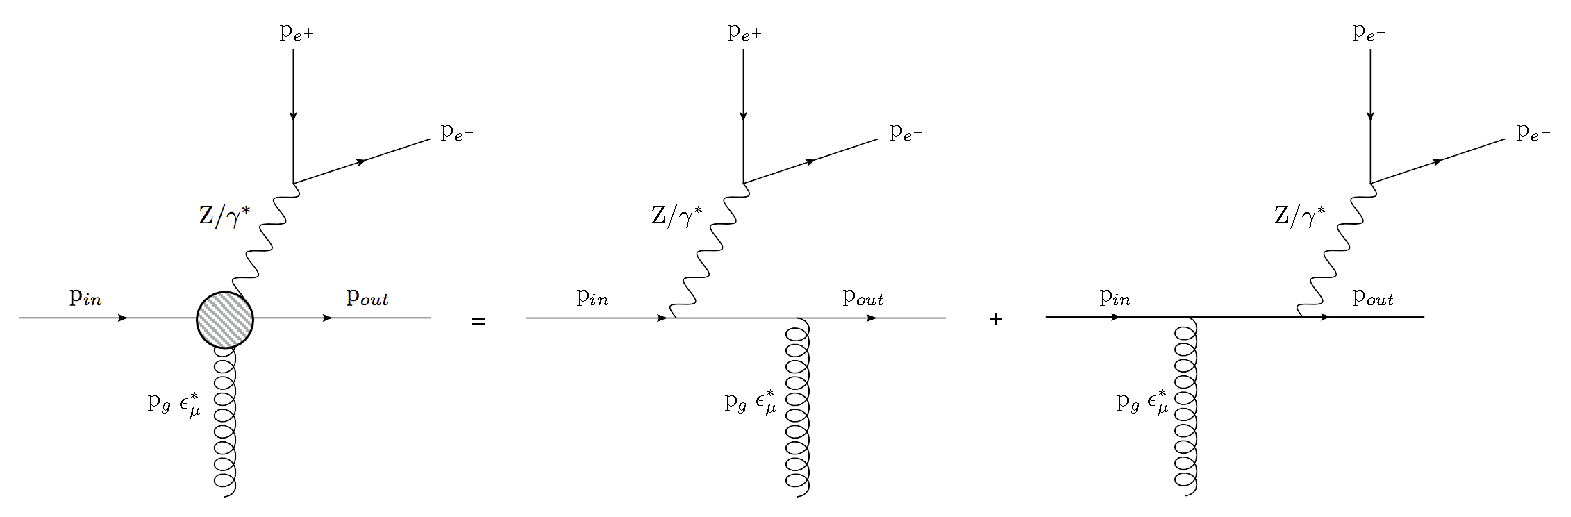
\includegraphics[width=0.98\linewidth]{figures/EmissionSites.pdf}
	\caption{The possible emission sites for a neutral weak boson.}
	\label{fig:emissionsites}
	\end{figure}

	In the language of currents (see for \emph{e.g.} \cite{Constructing}) we call
	the left hand side of fig. \ref{fig:emissionsites} $j_\mu^\zg$:

	\begin{equation}
		j_\mu^Z = \overline{u}^{h_{out}}(p_{out})\left(\gamma^\sigma\frac{\slashed p_{out} +
			\slashed p_Z}{(p_{out} + p_Z)^2}\gamma_\mu + \gamma_\mu\frac{\slashed p_{in} -
			\slashed p_Z}{(p_{in} - p_Z)^2}\gamma_\sigma\right)u^{h_{in}}(p_{in})\times
			\overline{u}^{h_{e^-}}(p_{e^-})\gamma_\sigma u^{h_{e^+}}(p_{e^+}).
	\end{equation}

	We can then express amplitudes in terms of contractions of `emitting' and `non-emitting'
	currents.\\As the fig. above indicates, when emitting a $Z$ boson there is also the
	possiblity of an off-shell photon being exchanged instead of a $Z$.  Since the difference
	in these two channels is indistinguishable in the final state we must treat the
	interference as the amplitude level.  For example, the amplitude for $2\rightarrow 2$ scattering is:

	\begin{equation}
	\mathcal{A}_{Z/\gamma}^{2\rightarrow 2} =\underbrace{\left(\frac{k_1}{p_{Z/\gamma}^2 - m^2_Z +
	i\Gamma_Zm_Z} + \frac{Q_1e}{p_{Z/\gamma}^2}\right)}_{\mathcal{K}_a}\frac{j^{Z/\gamma}_1\cdot
	j_2}{q_{t1}^2} + \underbrace{\left(\frac{k_2}{p_{Z/\gamma}^2 - m^2_Z + i\Gamma_Zm_Z} +
	\frac{Q_2e}{p_{Z/\gamma}^2}\right)}_{\mathcal{K}_b}\frac{j_1\cdot j^{Z/\gamma}_2}{q_{b1}^2},
	\label{eqn:2to2}
	\end{equation}

	where $k_i$ are the $Z$ couplings to the quarks, $Q_i$ are the the $\gamma$ couplings to
	the quarks, $m_Z$ is the mass of the $Z$, $\Gamma_Z$ is the width of the $Z$ peak, $q_{t1}$
	is the momentum of the $t$-channel gluon exchanged when $Z$ emission occurs of the forward
	incoming quark line and $q_{b1}$ is the momentum of the exchanged gluon when $Z$
	emission occurs of the backward incoming quark line.\\Eq. \eqref{eqn:2to2} is a
	good example of the advantages of using currents since the form of the diagrams for either
	$Z$ or $\gamma$ can be expressed as only two contraction (with the distinct propagators
	dealt with in the $\mathcal{K}_i$ terms).\\Extra \emph{real} gluon emissions from the
	$t$-channel gluon are then included using an effective vertex of the form \cite{JeppeHiggs}\cite{Constructing}:

	\begin{equation}
		V^\rho(q_j, q_{j+1}) = -(q_j + q_{j+1})^\rho - 2\left(\frac{s_{aj}}{s_{ab}} -
			\frac{q^2_{j+1}}{s_{bj}}\right)p_b^\rho + 2\left(\frac{s_{bj}}{s_{ab}} +
			\frac{q_j^2}{s_{aj}}\right)p_a^\rho,
			\label{eqn:effectivevertex}
	\end{equation}

	where $s_{aj} = 2p_a\cdot p_j$ \emph{etc.}  The general $2\rightarrow n$ amplitude therefore looks like:

	\begin{align}
		\mathcal{A}^{2\rightarrow n}_{Z/\gamma} = \Bigg(&\mathcal{K}_a\frac{V^{\mu_1}(q_{t1}, q_{t2})\cdots
			V^{\mu_{n-2}}(q_{t(n-1)}, q_{t(n-2)})} {q_{t1}\cdots q_{t(n-1)}} j_1^Z\cdot j_2 +\ldots\\\nonumber
			&\mathcal{K}_b\frac{V^{\mu_1}(q_{b1}, q_{b2})\cdots V^{\mu_{n-2}}(q_{b(n-1)}, q_{b(n-2)})} {q_{b1}
			\cdots q_{b(n-1)}} j_1  \cdot j_2^Z\Bigg)\epsilon^*_{\mu_1}\cdots\epsilon^*_{\mu_{(n-2)}}
	\end{align}

	and after taking the modulus squared of this we have the following:

	\begin{align}
	\begin{split}
		|\mathcal{A}_{Z/\gamma}^{2\rightarrow n}|^2 = \left|\mathcal{K}_a j_1^{Z/\gamma}\cdot j_2\right|^2
			\frac{V^2(q_{t1}, q_{t2}) V^2(q_{t2}, q_{t3}) \cdots V^2(q_{b(n-2)}, q_{b(n-1)})}{q^2_{t1}\cdots
			q^2_{t(n-1)}} +\ldots\\
			\left|\mathcal{K}_b j_2^{Z/\gamma}\cdot j_1\right|^2 \frac{V^2(q_{b1}, q_{b2}) V^2(q_{b2}, q_{b3})
			\cdots V^2(q_{b(n-2)}, q_{b(n-1)})}{q^2_{b1}\cdots q^2_{b(n-1)}} +\ldots\\
			2\Re\{\mathcal{K}_a\overline{\mathcal{K}_b} \times (j_1^{Z/\gamma}\cdot j_2)(\overline{j_2^{Z/\gamma}\cdot
			j_1})\}\frac{V(q_{t1}, q_{t2})\cdot V(q_{b1}, q_{b2})\cdots V(q_{t(n-2)}, q_{t(n-1)})\cdot V(q_{b(n-2)},
			q_{b(n-1)})}{q_{t1}q_{b1}\cdots q_{t(n-1)}q_{b(n-1)}}
			\label{eqn:interference}
	\end{split}
	\end{align}

	In previous work it was seen that the interference between forward quark- and backward weak boson emission
	(the third term in eq. \eqref{eqn:interference}) was negligible \cite{Wjets}.  This turns out not to be
	the case in $Z$ plus jets - possibly due to the effects of photon interference.

	\subsection{Formulation in terms of currents}

	\subsection{To High Multiplicity Final States}

	\subsection{$Z^0$ Emission Interference}

	\subsection{Photonic Interference}

	\subsection{The $2\rightarrow n$ Matrix Element}

	\subsection{The Differential ${Z/\gamma}$ Cross-Section}

\section{Regularising the $\zg$+Jets Matrix Element}
	\label{sec:regularising}

	Explain that in the MRK limit the external legs cant (by definition) be soft, then look at the limit
	of one gluon going soft (basically an NLO correction to the (n-1) parton ME) in the effective vertex.
	Show that this leads to a divergence.

	Next talk about NLO virtual corrections to the (n-1)-parton ME.  Show that in the HE limit, only two
	diagrams contribute (extra t - crosses and uncrossed - g exchange) show the log enhancement given.
	Give explicity calcultion showing divergences cancelling (as must happen by KLN theorem).

	\subsection{Soft Emissions}
	\label{sub:softEmissions}

		To calculate useful quantities such a cross sections \emph{etc.} we must integrate equation
		\eqref{eqn:interference} over all of phase space.  However, problems arise when we attempt to
		integrate over the so called `soft' (low energy) regions of phase space - things which should
		be finite diverge and need to be cancelled carefully.  It is well understood that the divergences
		coming from soft \emph{real} emissions cancel with those coming from soft \emph{virtual} emissions
		and so we must explicitly show this cancellation and calculate the remaining finite contribution
		multiplying the $(n-1)$-final state parton matrix element.\\In the previous work on $W^\pm$
		emission the finite contribution was found to be \cite{JeppeHiggs}\cite{Constructing}:

		\begin{equation}
			\frac{\alpha_s C_a \Delta_{j-1, j+1}}{\pi}\ln{\frac{\lambda^2}{|\vec{q}_{j\perp}|^2}},
		\end{equation}

		where $\alpha_s$ is the strong coupling strength, $C_a$ is a numerical factor, $\Delta_{i-1, i+1}$
		is the rapidity span of the final state partons either side of our soft emission, $\lambda$ is a
		factor chosen to define the soft region: $p^2 < \lambda^2$ and $|\vec{q}_{j\perp}|^2$ is the sum of
		squares of the transverse components of the $j^{th}$ $t$-channel gluon momenta.\\Here we investigate
		the cancellation of these divergences for $Z$ emission and most importantly whether the finite term
		is of the same form for the interference term which was previous disregarded.\\We start by looking
		at a $2\rightarrow n$ process and take the limit of one final state parton momentum, $p_i$, becoming
		small.  Because of the form of eq. \eqref{eqn:interference} this ammounts to looking at the
		effect of soft-ness on eq. \eqref{eqn:effectivevertex}, we can immediately see that for $p_i$
		going soft the gluon chain momenta coming into- and coming out of the $j^{th}$ emission site will
		coincide: $q_{j+1}\sim q_j$:

		\begin{equation}
			V^\rho(q_j, q_{j+1}) \rightarrow -2q_j^\rho - 2\left(\frac{s_{aj}}{s_{ab}} -
				\frac{q^2_{j}}{s_{bj}}\right)p_b^\rho + 2\left(\frac{s_{bj}}{s_{ab}} +
				\frac{q_j^2}{s_{aj}}\right)p_a^\rho
				\label{eqn:vertexlimit}
		\end{equation}

		In eq. \eqref{eqn:interference} we have two types of terms involving the effective vertex;
		terms like $V^2(q_{t/bj}, q_{t/b(j+1)})$ and terms like $V(q_{tj}, q_{t(j+1)})\cdot V(q_{bj}, q_{b(j+1)})$.
		The procedure for the $V^2$ terms doesnt not change between top-line emission and bottom-line emission
		and so only the calculation for top-line emission will be shown here.

	\subsection{$V^2(q_{tj}, q_{t(j+1)})$ Terms}
	\label{sub:subsection_name}

		Once we square eq. \eqref{eqn:vertexlimit} and impose on-shell conditions to $p_a$ and $p_b$ we get:

		\begin{equation}
			V^2(q_{tj}, q_{tj}) = 4q_j^2 + 8 q_j\cdot p_b \left(\frac{s_{aj}}{s_{ab}} - \frac{q^2_{j}}{s_{bj}}\right) -
				8q_j\cdot p_a \left(\frac{s_{bj}}{s_{ab}} + \frac{q_j^2}{s_{aj}}\right) - 4s_{ab}\left(\frac{s_{aj}}{s_{ab}} -
				\frac{q^2_{j}}{s_{bj}}\right)\left(\frac{s_{bj}}{s_{ab}} + \frac{q_j^2}{s_{aj}}\right)
		\end{equation}

		Now since $p_j\rightarrow0$ the terms $s_{aj}$ and $s_{bj}$ will also become vanishing:

		\begin{equation}
			V^2(q_{tj}, q_{tj}) = 4q_j^2 + 8 q_j\cdot p_b \frac{q^2_{j}}{s_{bj}} - 8 q_j\cdot p_a \frac{q_j^2}{s_{aj}} -
				4s_{ab}\frac{q^4_{j}}{s_{bj}s_{aj}}
		\end{equation}

		Clearly the final term now dominates due to its $\sim\frac{1}{p_i^2}$ behaviour:

		\begin{equation}
			V^2(q_{ti}, q_{ti}) = - \frac{4s_{ab}}{s_{bi}s_{ai}}q^4_{i} + \mathcal{O}\left(\frac{1}{|p_i|}\right)
			\label{eqn:temp}
		\end{equation}

		We must now explicitly calculate the invariant mass terms.  Since we are in the high energy limit we may take
		$p_a\sim p_1 \sim p_+ = (\frac12 p_z, 0, 0, \frac12 p_z)$ and $p_b\sim p_n \sim p_- = (\frac12 p_z, 0, 0, -\frac12 p_z)$
		and we describe our soft gluon by $p_i=(E, \vec{p})$.  Therefore:

		\begin{subequations}
			\begin{equation}
				s_{ai} = 2p_a\cdot p_i\sim2p_+\cdot p_i = \frac12p_zE - \frac12p_z^2,
			\end{equation}
			\begin{equation}
				s_{bi} = 2p_b\cdot p_i\sim2p_-\cdot p_i = \frac12p_zE + \frac12p_z^2,
			\end{equation}
		\end{subequations}

		and $s_{ab}=\frac12p_z^2$.  Then eq. \eqref{eqn:temp} reads:

		\begin{subequations}
			\begin{equation}
			V^2(q_{ti}, q_{ti}) = - \frac{4p_z^2}{(p_zE - p_z^2)(p_zE + p_z^2)}q^4_{i} + \mathcal{O}\left(\frac{1}{|p_i|}\right),
			\end{equation}
			\begin{equation}
			V^2(q_{ti}, q_{ti}) = - \frac{4p_z^2}{p_z^2(E^2-p_z^2)}q^4_{i} + \mathcal{O}\left(\frac{1}{|p_i|}\right),
			\end{equation}
		\end{subequations}

		but since $E^2-\vec{p}_1^2=0$:

		\begin{equation}
			V^2(q_{ti}, q_{ti}) = - \frac{4}{|\vec{p}_{1\perp}|^2}q^4_{i} + \mathcal{O}\left(\frac{1}{|p_i|}\right),
			\label{eqn:temp2}
		\end{equation}

		Now looking back to eq. \eqref{eqn:interference} we see that each vertex is associated with factors of
		$(q^{-2}_{ti}q^{-2}_{t(i+1)})$ but once again since the emission is soft this becomes $(q^{-4}_{ti}$.
		This factor conspires to cancel with that in eq. \eqref{eqn:temp2}, moreover each vertex comes with a
		factor of $-C_Ag^2_s$ (which are contained in the $\mathcal{K}_i$ terms in eq. \eqref{eqn:interference}).
		Including these and dropping subdominant terms the final factor is:

		\begin{equation}
			\frac{4C_Ag_s^2}{|\vec{p}_\perp|^2}
			\label{eqn:finalsoft}
		\end{equation}

	\subsection{$V(q_{ti}, q_{t(i+1)})\cdot V(q_{bi}, q_{b(i+1)})$ Terms}
	\label{sub:subsection_name}

		The calculation of the interference term with a soft emission follows similarly to the above section.
		After taking $p_i\rightarrow0$ and dotting the two vertex terms together we have:

		\begin{equation}
		\begin{split}
			V(q_{ti}, q_{ti})\cdot V(q_{bi}, q_{bi}) = 4q_i^t\cdot q_i^b &- 4q_i^t\cdot p_a\left(\frac{s_{bi}}{s_{ab}} +
				\frac{t_i^b}{s_{ai}}\right) + 4q_i^t\cdot p_b\left(\frac{s_{ai}}{s_{ab}} + \frac{t_i^b}{s_{bi}}\right) \ldots\\
				&- 4q_i^b\cdot p_a\left(\frac{s_{bi}}{s_{ab}} + \frac{t_i^t}{s_{ai}}\right) +
				4q_i^b\cdot p_b\left(\frac{s_{ai}}{s_{ab}} +
				\frac{t_i^t}{s_{bi}}\right) \ldots\\
		\end{split}
		\end{equation}

		having use $p_a^2=0$ and $p_b^2=0$ once again.  We can drop all the terms with $s_{ai}$ or
		$s_{bi}$ in the denominator and this time we are left with \emph{two} dominant terms which
		combine to give:

		\begin{equation}
			V(q_{ti}, q_{ti})\cdot V(q_{bi}, q_{bi}) = -\frac{s_{ab}}{s_{ai}s_{bi}}t_i^tt_i^b +
				\mathcal{O}\left(\frac{1}{|p_i|}\right).
		\end{equation}

		The invariant mass terms here are identical to those we say in the $V^2$ terms and the products of
		$t_i^tt_i^b$ also appear in the denominator of the interference term in eq. \eqref{eqn:interference}.
		After this cancelling we are left with exactly what we had before (see eq. \eqref{eqn:finalsoft}).
		Since exactly the same factor comes from all three terms at the amplitude squared level we may factor
		them out and express the amplitude squared for an $n$-parton final state with one soft emission in
		terms of an $(n-1)$-parton final state amplitude squared multiplied by our factor:

		\begin{equation}
			\lim_{p_i\rightarrow0} |\mathcal{A}_{Z/\gamma}^{2\rightarrow n}|^2 = \left(\frac{4C_Ag_s^2}{|\vec{p}_{i\perp}|^2}\right)
				|\mathcal{A}_{Z/\gamma}^{2\rightarrow (n-1)}|^2
		\end{equation}

	\subsection{Integration of soft diverences}
	\label{sub:subsection_name}

		As mentioned above the divergences only become apparent after we have attempted to integrate over
		phase space.  The Lorentz invariant phase space integral associated with $p_i$ is:

		\begin{equation}
			\int\frac{d^3\vec{p_i}}{(2\pi)^32E_i}\frac{4C_Ag_s^2}{|\vec{p}_\perp|^2}.
		\end{equation}

		It is convenient to replace the integral over the $z$-component of momentum with one over rapidity,
		$y_2$.  Rapidty and momentum are realted through:

		\begin{equation}
			y = \frac12\ln\left(\frac{E + p_z}{E - p_z}\right)
		\end{equation}

		The Jacobian of this transformation is:

		\begin{align}
			\frac{dy}{dp_z} &= \frac{1}{2(E+p_z)} \frac{\partial}{\partial p_z}(E+p_z) - \frac{1}{2(E-p_z)}\frac{\partial}{\partial p_z}(E-p_z),\\
			&= \frac{E}{E^2-p_z^2} - \frac{p_z}{E^2-p_z^2}\frac{\partial E}{\partial p_z},\\
			&= \frac{E}{E^2-p_z^2} - \frac{p_z}{E^2-p_z^2}\frac{p_z}{E},\\
			&= \frac{1}{E}.
		\end{align}

		The phase space integral then reads:

		\begin{equation}
			\int\frac{d^{2+2\epsilon}\vec{p}_{\perp}}{(2\pi)^{2+2\epsilon}}\frac{dy}{4\pi}\frac{4C_Ag_s^2}
				{|\vec{p}_\perp|^2}\mu^{-2\epsilon} = \frac{4C_Ag_s^2\mu^{-2\epsilon}}{(2\pi)^{2+2\epsilon}4\pi}
				\Delta_{i-1, i+1}\int\frac{d^{2+2\epsilon}\vec{p}_{\perp}}{|\vec{p}_\perp|^2},
		\end{equation}

		where we have analytically continued the integral to $2+2\epsilon$ dimensions to regulate the
		divergence and introduced the parameter $\mu$ to keep the coupling dimensionless in the process.
		Converting to polar cooerdinates and using the result for the volume of a unit hypersphere gives
		to integrated soft contribution:

		\begin{equation}
			\frac{4C_Ag_s^2}{(2\pi)^{2+2\epsilon}4\pi}\Delta_{i-1, i+1}\frac{1}{\epsilon}\frac{\pi^{1+\epsilon}}
				{\Gamma(\epsilon+1)}\left(\frac{\lambda^2}{\mu^2}\right)^\epsilon
				\label{eqn:soft}
		\end{equation}

	\subsection{Virtual Emissions}
	\label{sub:subsection_name}

		The virtual emission diagrams are included using the Lipatov ansatz for the gluon propagator:

		\begin{equation}
			\frac{1}{q_i^2}\longrightarrow\frac{1}{q_i^2}e^{\hat{\alpha}(q_i)(\Delta_{i,i-1})},
		\end{equation}

		where:

		\begin{equation}
			\hat{\alpha}(q_i) = \alpha_sC_Aq_i^2\int \frac{d^{2+2\epsilon}k_{\perp}}{(2\pi)^{2+2\epsilon}}
			\frac{1}{k^2_\perp(k_\perp - q_{i\perp})^2}\mu^{-2\epsilon}.
		\end{equation}

		Once again we choose to perform the integral using dimensional regularistion.
		Using the well known Feynman parameterisation formulae gvies:

		\begin{align}
			\hat{\alpha}(q_i) &= \alpha_sC_Aq_i^2\int \frac{d^{2+2\epsilon}k_{\perp}}{(2\pi)^{2+2\epsilon}}\int_0^1
				\frac{dx}{[x(k - q_{i})^2_\perp + (1-x)k_\perp^2]^2}\mu^{-2\epsilon}, \\
				&= \alpha_sC_Aq_i^2\int \frac{d^{2+2\epsilon}\hat{k}_{\perp}}{(2\pi)^{2+2\epsilon}}\int_0^1
				\frac{dx}{[\hat{k}^2 _\perp + q_{i\perp}^2(1-x)]^2}\mu^{-2\epsilon},
		\end{align}

		where we have performed a change of variables to $\hat{k}_\perp = k_\perp - xq_{i\perp}$ with
		unit Jacobian.  Changing the order of integration we can perform the $\hat{k}_\perp$ integral
		using the following result:

		\begin{equation}
			\int \frac{d^dk}{(2\pi)^d}\frac{1}{(k^2 - C)^\alpha} = \frac{1}{(4\pi)^{\frac{d}{2}}}
				\frac{\Gamma(\alpha - \frac{d}{2})}{\Gamma(\alpha)}\frac{(-1)^\alpha}{C^{\alpha - \frac{d}{2}}},
		\end{equation}

		to give:

		\begin{align}
			\hat{\alpha}(q_i) &= \alpha_sC_Aq_i^2\frac{\Gamma(1-\epsilon)}{(4\pi)^{1+\epsilon}}(-q_{i\perp}^2)^{\epsilon-1}
				\int_0^1 dx(1-x)^{\epsilon-1}, \\
				&= -\frac{2g_s^2C_A}{(4\pi)^{2+\epsilon}}\frac{\Gamma(1-\epsilon)}{\epsilon}\left(\frac{q_{i\perp}^2}{\mu^2}\right)^\epsilon,
		\end{align}

		having completed the $x$ integral and used $\alpha_s=\frac{g_s^2}{4\pi}$.

	\subsection{Cancellation of Infrared Contributions}
	\label{sub:subsection_name}

		We now show how the infrared contributions from soft real emissions and virtual emissions cancel leaving
		our integrated matrix element finite.  The subtlety here is that we must sum two diagrams with different
		final states to see the cancellation.  This is because they are experimentally indistinguishable;
		the $2\rightarrow (n-1)$ virtual diagram has $(n-1)$ resolvable partons in the final state (but is a
		higher order diagram perturbatively speaking).  Because on of the emission in the real $2\rightarrow n$
		diagram is soft it is experimentally undetectable so we detect the same final state as the virtual diagram.
		The matrix element squared for the real soft diagram will look like:

		\begin{align}
			|\mathcal{A}_{Z/\gamma}^{2\rightarrow n}|^2 = \left(\frac{4g_s^2C_a}{|p_{i\perp}|^2}\right)
				\Bigg[&\left|\mathcal{K}_a j_1^{Z/\gamma}\cdot j_2\right|^2 \frac{\prod^{n-2}_{i\neq j}V^2(q_{ti},
				q_{t(i+1)})}{\prod^{n-1}_{i\neq j}q^2_{ti}} + \ldots \\&\left|\mathcal{K}_b j_2^{Z/\gamma}\cdot j_1\right|^2
				\frac{\prod^{n-2}_{i\neq j}V^2(q_{bi}, q_{b(i+1)})}{\prod^{n-1}_{i\neq j}q^2_{bi}} + \ldots \\
				&2\Re\{\mathcal{K}_a\overline{\mathcal{K}_b} \times (j_1^{Z/\gamma}\cdot j_2)(\overline{j_2^{Z/\gamma}\cdot j_1})\}
				\frac{\prod^{n-2}_{i\neq j}V(q_{ti}, q_{t(i+1)})\cdot V(q_{bi}, q_{b(i+1)}))}{\prod^{n-1}_{i\neq j}q_{ti}q_{bi}}\Bigg],
		\end{align}

		where we have taken the $i^{th}$ gluon to be soft and the result of the Lorentz invariant phase space
		integration over the $p_i$ momentum is shown in eq. \eqref{eqn:soft}.\\After inserting the Lipatov
		ansatz into the $2\rightarrow (n-1)$ matrix element squared we have:

		\begin{align}
			|\mathcal{A}_{Z/\gamma}^{2\rightarrow (n-1)}|^2 = &\left|\mathcal{K}_a j_1^{Z/\gamma}\cdot j_2\right|^2
				\frac{\prod^{n-3}_{i}V^2(q_{ti}, q_{t(i+1)})}{\prod^{n-2}_{i}q^2_{ti}}e^{2\hat{\alpha}(q_{ti})\Delta_{i-1,i+1}} + \ldots \\
				&\left|\mathcal{K}_b j_2^{Z/\gamma}\cdot j_1\right|^2 \frac{\prod^{n-3}_{i}V^2(q_{bi}, q_{b(i+1)})}
				{\prod^{n-2}_{i}q^2_{bi}}e^{2\hat{\alpha}(q_{bi})\Delta_{i-1,i+1}} + \ldots \\
				&2\Re\{\mathcal{K}_a\overline{\mathcal{K}_b} \times (j_1^{Z/\gamma}\cdot j_2)(\overline{j_2^{Z/\gamma}\cdot j_1})\}
				\frac{\prod^{n-3}_{i}V(q_{ti}, q_{t(i+1)})\cdot V(q_{bi}, q_{b(i+1)}))}{\prod^{n-2}_{i}q_{ti}q_{bi}}
				e^{(\hat{\alpha}(q_{bi}) + \hat{\alpha}(q_{bi}))\Delta_{i-1,i+1}},
		\end{align}

		We can now go through term-by-term to show the divergences cancel and find the finite contribution to
		the matrix element squared.  Similarly to when we calculated the soft terms the pure top and bottom
		emissions follow identically so here we will only state the procedure for the top emission.  The
		interference term is slightly different.\\For the top line emission we have the following terms:

		\begin{equation}
			\frac{4C_Ag_s^2}{(2\pi)^{2+2\epsilon}4\pi}\Delta_{i-1, i+1}\frac{1}{\epsilon}\frac{\pi^{1+\epsilon}}
			{\Gamma(\epsilon+1)}\left(\frac{\lambda^2}{\mu^2}\right)^\epsilon + e^{2\hat{\alpha_s}(q_{ti})\Delta_{i-1,i+1}}.
		\end{equation}

		We now extract the relevant term (in terms of the strong coupling order) from the
		exponential and substitute the expression for $\hat{\alpha_s}$:

		\begin{align}
			&= \frac{4C_Ag_s^2}{(2\pi)^{2+2\epsilon}4\pi}\Delta_{i-1, i+1}\frac{1}{\epsilon}\frac{\pi^{1+\epsilon}}
			{\Gamma(\epsilon+1)}\left(\frac{\lambda^2}{\mu^2}\right)^\epsilon - -\frac{2g_s^2C_A}{(4\pi)^{2+\epsilon}}
			\frac{\Gamma(1-\epsilon)}{\epsilon}\left(\frac{q_{ti\perp}^2}{\mu^2}\right)^\epsilon, \\
			&= \frac{g_s^2C_A}{4^{1+\epsilon}\pi^{2+\epsilon}}\Delta_{i-1, i+1}\left(\frac{1}{\epsilon\Gamma(1+\epsilon)}
			\left(\frac{\lambda^2}{\mu^2}\right)^\epsilon - \frac{\Gamma(1-\epsilon)}{\epsilon}
			\left(\frac{q_{ti\perp}^2}{\mu^2}\right)^\epsilon\right).
		\end{align}

		Expanding the terms involving $\epsilon$ yeilds:

		\begin{subequations}
		\begin{equation}
		\frac{1}{\Gamma(1+\epsilon)} = 1 + \gamma_E\epsilon + \mathcal{O}(\epsilon^2),
		\end{equation}
		\begin{equation}
		\Gamma(1-\epsilon) = 1 + \gamma_E\epsilon + \mathcal{O}(\epsilon^2),
		\end{equation}
		\begin{equation}
		\left(\frac{x}{y}\right)^\epsilon = 1 + \epsilon\ln\left(\frac{x}{y}\right) + \mathcal{O}(\epsilon^2).
		\end{equation}
		\end{subequations}

		And so the finite terms are:

		\begin{subequations}
			\begin{equation}
				= \frac{g_s^2C_A\Delta_{i-1, i+1}}{4^{1+\epsilon}\pi^{2+\epsilon}}\left((1 + \gamma_E\epsilon +
				\mathcal{O}(\epsilon^2))\left(\frac{1}{\epsilon} + \ln\left(\frac{\lambda^2}{\mu^2}\right) +
				\mathcal{O}(\epsilon)\right) - (1 + \gamma_E\epsilon + \mathcal{O}(\epsilon^2))\left(\frac{1}{\epsilon} +
				\ln\left(\frac{q_{ti\perp}^2}{\mu^2}\right) + \mathcal{O}(\epsilon)\right)\right)\\
			\end{equation}
				\begin{equation}
				= \frac{g_s^2C_A\Delta_{i-1, i+1}}{4\pi^2}\ln\left(\frac{\lambda^2}{q_{ti\perp}^2}\right)\\
				\end{equation}
				\begin{equation}
				= \frac{\alpha_sC_A\Delta_{i-1, i+1}}{\pi}\ln\left(\frac{\lambda^2}{q_{ti\perp}^2}\right)
			\end{equation}
		\end{subequations}

		Likewise for the emission purely from the backward quark line we have:

		\begin{equation}
		= \frac{\alpha_sC_A\Delta_{i-1, i+1}}{\pi}\ln\left(\frac{\lambda^2}{q_{bi\perp}^2}\right)
		\end{equation}

		For the interference we expand the exponential with both forward emission $q$
		momenta and backward emission $q$ momenta to get:

		\begin{subequations}
			\begin{equation}
				= \frac{g_s^2C_A\Delta_{i-1, i+1}}{4^{1+\epsilon}\pi^{2+\epsilon}}\left(\left(\frac{1}{\epsilon} +
				\gamma_E +  \ln\left(\frac{\lambda^2}{\mu^2}\right) + \mathcal{O}(\epsilon)\right) - \frac{1}{2}
				\left[\frac{2}{\epsilon} + 2 \gamma_E + \ln\left(\frac{q_{ti\perp}^2}{\mu^2}\right) -
				\ln\left(\frac{q_{bi\perp}^2}{\mu^2}\right) + \mathcal{O}(\epsilon)\right]\right) \\
			\end{equation}
			\begin{equation}
				= \frac{\alpha_sC_A\Delta_{i-1, i+1}}{\pi}\ln\left(\frac{\lambda^2}{\sqrt{q_{ti\perp}^2q_{bi\perp}^2}}\right)
			\end{equation}
		\end{subequations}

		This is a very similar form to that found in \cite{Constructing} and \cite{JeppeHiggs}.

	\subsection{Example: $2\rightarrow4$ Scattering}
	\label{sub:2to4Example}

	\begin{figure}[bth!]

		\centering

		\begin{subfigure}[b]{0.5\textwidth}
			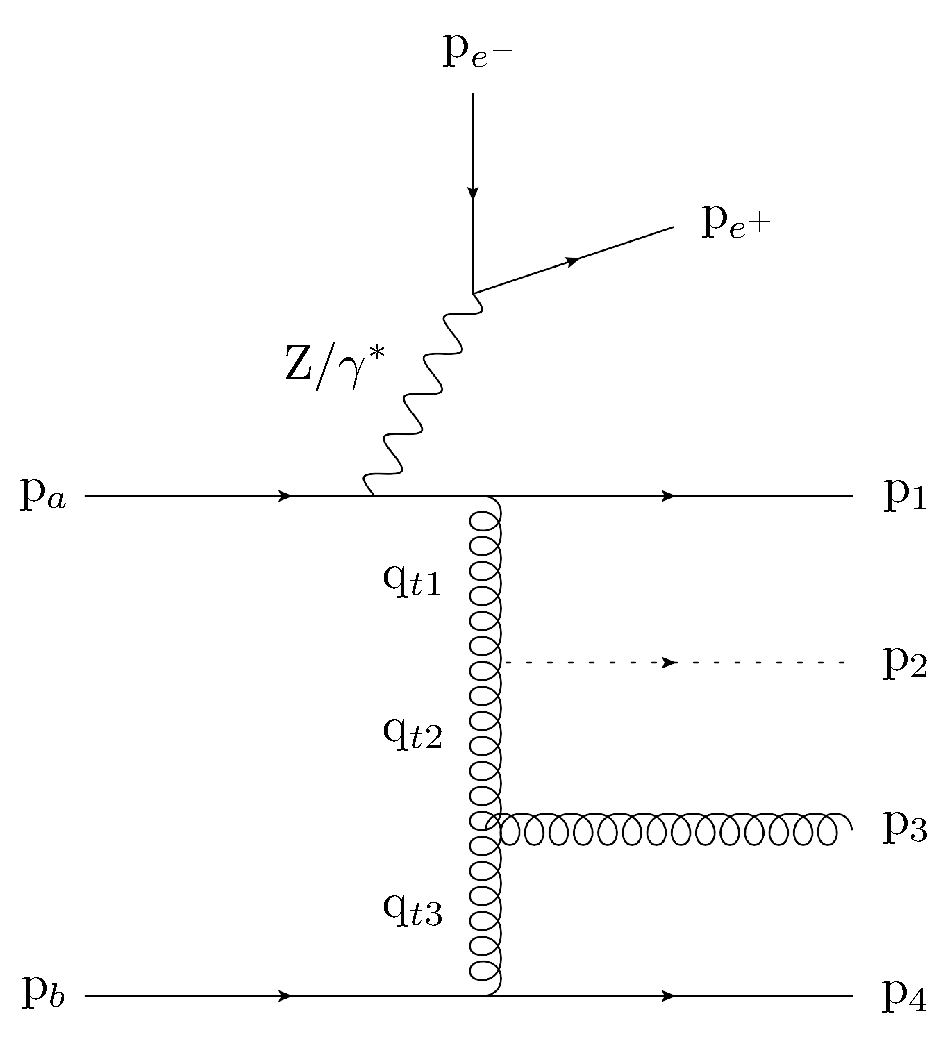
\includegraphics[width=1.0\linewidth]{RealSoftEmissionZ.pdf}
			\caption{Soft Emission}
			\label{fig:real24}
		\end{subfigure}

		\begin{subfigure}[b]{0.5\textwidth}
			\centering
			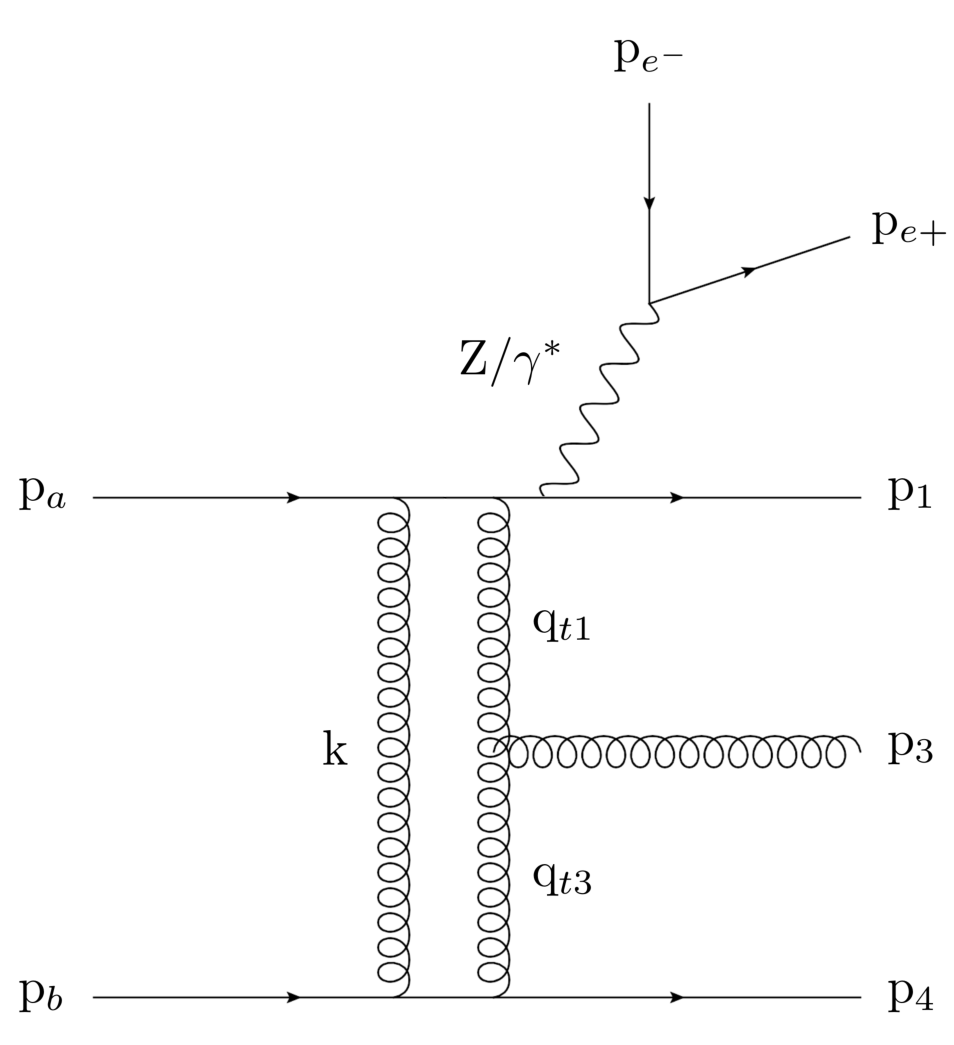
\includegraphics[width=1.0\linewidth]{VirtualSoftEmissionZ.pdf}
			\caption{Virtual Emission}
			\label{fig:virtual24}
		\end{subfigure}

		\caption{Examples of diagrams contributing to $2\rightarrow4$ scattering.
		In fig. \ref{fig:real24} the $p_2$ has been drawn with a dashed line to denote
		it is not resolvable.  In fig. \ref{fig:virtual24} the final state momenta have
		been labelled in a seemingly strange way - this was done to make clear the
		cancellation when working through the algebra.}

		\label{fig:2to4}
	\end{figure}

	As an example we show the cancellation explicitly for the case of $2\rightarrow4$ when the
	$p_2$ momentum has gone soft.  A contributing soft diagram is shown in fig. \ref{fig:real24} and
	one example of a contributing virtual diagram of the same order is shown in fig. \ref{fig:virtual24}.
	When $p_2$ goes soft we have the following form for the $2\rightarrow4$ integrated amplitude squared
	({N.B.}: The integration is only schematic and doesnt represent the full Lorentz invariant phase space):

	\begin{align}
	\begin{split}
		\int|\mathcal{A}^{2\rightarrow4}_{soft}|^2 = &\frac{4C_Ag_s^2\Delta_{1,3}}{(2\pi)^{2+2\epsilon}4\pi}
		\frac{\pi^{\epsilon+1}}{\epsilon\Gamma(\epsilon+1)}
		\left(\frac{\lambda^2}{\mu^2}\right)^\epsilon\Bigg[|\mathcal{K}_aj_1^Z\cdot j_2|^2
		\frac{V^2(q_{t1}, q_{t3})}{q^2_{t1}q^2_{t3}} + |\mathcal{K}_bj_1\cdot j_2^Z|^2
		\frac{V^2(q_{b1}, q_{b3})}{q^2_{b1}q^2_{b3}} + \ldots \\
		& 2\Re\left\{\mathcal{K}_a\overline{\mathcal{K}_b}
		(j_1^Z\cdot j_2)\overline{(j_1\cdot j_2^Z)}\right\} \frac{V(q_{t1}, q_{t3})
		\cdot V(q_{b1}, q_{b3})}{q_{t1}q_{t3}q_{b1}q_{b3}}\Bigg],
	\end{split}
	\end{align}

	and the virtual contributions for the $2\rightarrow3$ amplitude is:

	\begin{align}
	\begin{split}
		\int|\mathcal{A}^{2\rightarrow3}_{virtual}|^2 = &|\mathcal{K}_bj_1\cdot j_2^Z|^2
		\frac{V^2(q_{t1}, q_{t3})}{q_{t1}^2}e^{2\hat{\alpha}(q_{t1})\Delta_{1,3}} +
		|\mathcal{K}_tj_1^Z\cdot j_2|^2 \frac{V^2(q_{b1}, q_{b3})}{q_{b1}^2}e^{2\hat{\alpha}(q_{b1})\Delta_{1,3}} + \ldots \\
		& 2\Re\left\{\mathcal{K}_a\overline{\mathcal{K}_b}  (j_1^Z\cdot j_2)\overline{(j_1\cdot j_2^Z)}\right\}
		\frac{V(q_{t1}, q_{t3})\cdot V(q_{b1}, q_{b3})}{q_{t1}q_{t3}q_{b1}q_{b3}}e^{(\hat{\alpha}(q_{t1}) +
		\hat{\alpha}(q_{b1}))\Delta_{1,3}}.
	\end{split}
	\end{align}

	Once we expand the exponential to the correct order in $g_s^2$, the sum of these
	matrix elements squared over the region of phase space when $p_2$ is soft is:

	\begin{align}
	\begin{split}
		\int\left(|\mathcal{A}^{2\rightarrow4}_{soft}|^2 + |\mathcal{A}^{2\rightarrow3}_{virtual}|^2\right) =
		&|\mathcal{K}_aj_1^Z\cdot j_2|^2 \frac{V^2(q_{t1}, q_{t3})}{q_{t1}^2}
		{\Bigg(\frac{4C_Ag_s^2\Delta_{1,3}}{(2\pi)^{2+2\epsilon}4\pi}\frac{\pi^{\epsilon+1}}
		{\epsilon\Gamma(\epsilon+1)} - 2\hat{\alpha}(q_{t1})\Delta_{1,3}\Bigg)}+\ldots \\
		& |\mathcal{K}_bj_1\cdot j_2^Z|^2 \frac{V^2(q_{b1}, q_{b3})}{q_{b1}^2}
		{\Bigg(\frac{4C_Ag_s^2\Delta_{1,3}}{(2\pi)^{2+2\epsilon}4\pi}\frac{\pi^{\epsilon+1}}
		{\epsilon\Gamma(\epsilon+1)} - 2\hat{\alpha}(q_{b1})\Delta_{1,3}\Bigg)}+\ldots \\
		2\Re\left\{\mathcal{K}_a\overline{\mathcal{K}_b}  (j_1^Z\cdot j_2)\overline{(j_1\cdot j_2^Z)}\right\}&
		\frac{V(q_{t1}, q_{t3})\cdot V(q_{b1}, q_{b3})}{q_{t1}q_{t3}q_{b1}q_{b3}}{\Bigg(\frac{4C_Ag_s^2\Delta_{1,3}}
		{(2\pi)^{2+2\epsilon}4\pi}\frac{\pi^{\epsilon+1}}{\epsilon\Gamma(\epsilon+1)} -
		(\hat{\alpha}(q_{t1}) + \hat{\alpha}(q_{b1}))\Delta_{1,3}\Bigg)} + \mathcal{O}(g_s^4),\\
	\end{split}
	\end{align}

	These bracketed terms are exactly the cancellations calculated in section 4 above.  Therefore:

	\begin{align}
	\begin{split}
		\int\left(|\mathcal{A}^{2\rightarrow4}_{soft}|^2 + |\mathcal{A}^{2\rightarrow3}_{virtual}|^2\right) =
		\frac{\alpha_sC_A\Delta_{1,3}}{\pi}\Bigg(&|\mathcal{K}_aj_1^Z\cdot j_2|^2 \frac{V^2(q_{t1},
		q_{t3})}{q_{t1}^2}\ln\left(\frac{\lambda^2}{|q_{1t\perp}|^2}\right)+\ldots \\
		& |\mathcal{K}_bj_1\cdot j_2^Z|^2 \frac{V^2(q_{b1}, q_{b3})}{q_{b1}^2}\ln
		\left(\frac{\lambda^2}{|q_{1b\perp}|^2}\right)+\ldots \\
		2\Re\left\{\mathcal{K}_a\overline{\mathcal{K}_b}  (j_1^Z\cdot j_2)\overline{(j_1\cdot j_2^Z)}\right\}
		&\frac{V(q_{t1}, q_{t3})\cdot V(q_{b1}, q_{b3})}{q_{t1}q_{t3}q_{b1}q_{b3}}\ln
		\left(\frac{\lambda^2}{\sqrt{|q_{1t\perp}|^2|q_{1b\perp}|^2}}\right)\Bigg) + \mathcal{O}(\alpha_s^2),\\
	\end{split}
	\end{align}

	Which is manifestly finite.

\section{Subtractions and the $\lambda_{cut}$ scale}
	\label{sec:indep-lambd}

	The table below shows the value of the total cross section for varying values of
	the parameter $\lambda_{cut}$ defined in section~\ref{sec:Constructing}.  It is
	clear that the cross section does not display a large dependence on the value of $\lambda_{cut}$.
	Figure~\ref{fig:lambdadist} shows the effect of the same variation in $\lambda_{cut}$ on the
	differential distribution in the rapidity gap between the two leading jets in $p_\perp$.
	Our default chosen value is 0.2.

	\begin{table}[htp!]
	\begin{center}
		\begin{tabular}{| c | c | c | c |}
		\hline
		$\lambda_{cut}$ (GeV) & $\sigma(2j)$ ($pb$) & $\sigma(3j)$ ($pb$) & $\sigma(4j)$ ($pb$) \\ \hline
		0.2 & $5.03 \pm 0.02$ & $0.70 \pm 0.02$ & $0.13 \pm 0.03$ \\
		0.5 & $5.05 \pm 0.01$ & $0.70 \pm 0.01$ & $0.13 \pm 0.01$ \\
		1.0 & $5.09 \pm 0.01$ & $0.71 \pm 0.01$ & $0.13 \pm 0.01$ \\
		2.0 & $5.16 \pm 0.04$ & $0.72 \pm 0.01$ & $0.13 \pm 0.01$ \\ \hline
		\end{tabular}
		\caption{The total cross-sections for the 2, 3 and 4 jet exclusive rates with associated
		         statistical errors shown for different values of the regularisation parameter $\lambda_{cut}$.
		         The scale choice was the half the sum over all traverse scales in the event, $H_T/2$.}
	\end{center}
	\end{table}

	\begin{figure}[htp!]
		\centering
		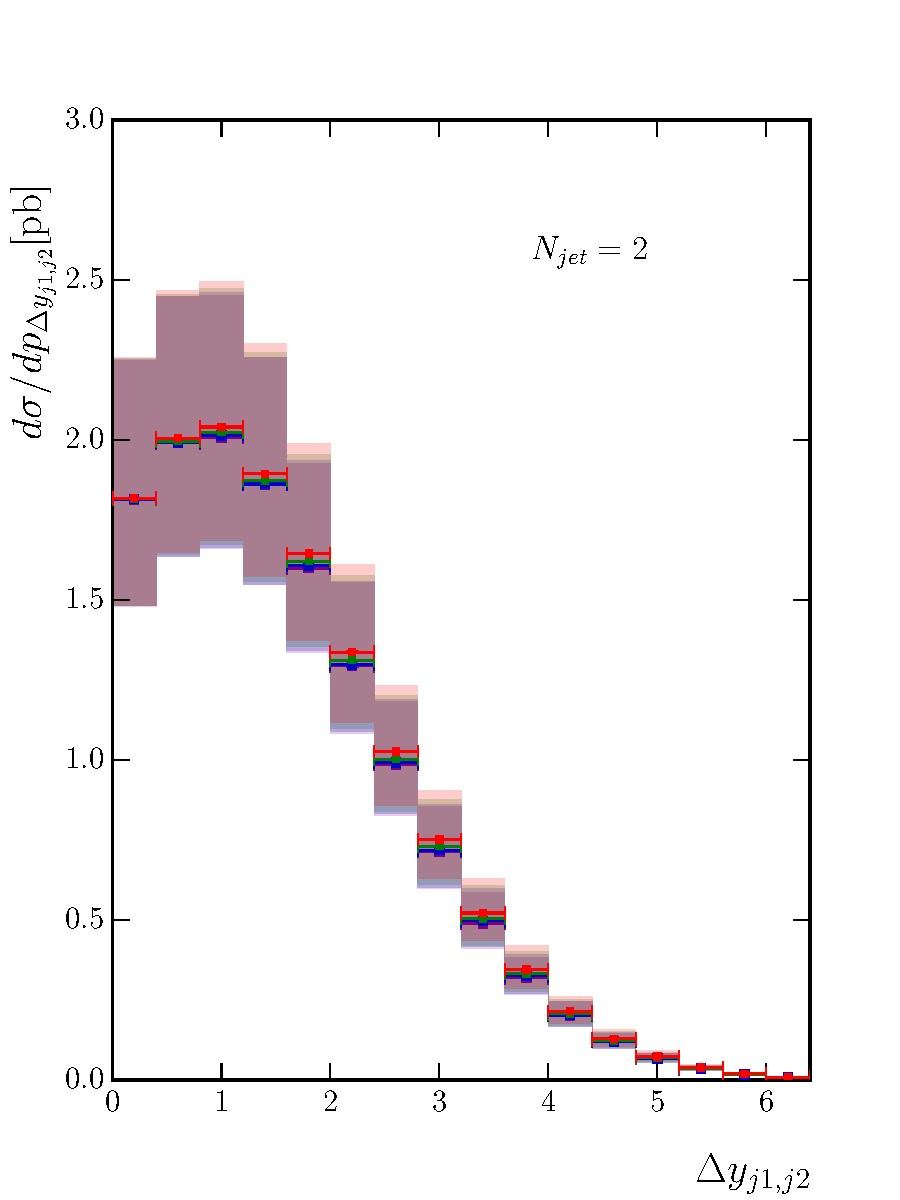
\includegraphics[width=.5\textwidth]{Z_11a_2j.pdf}\hfill
		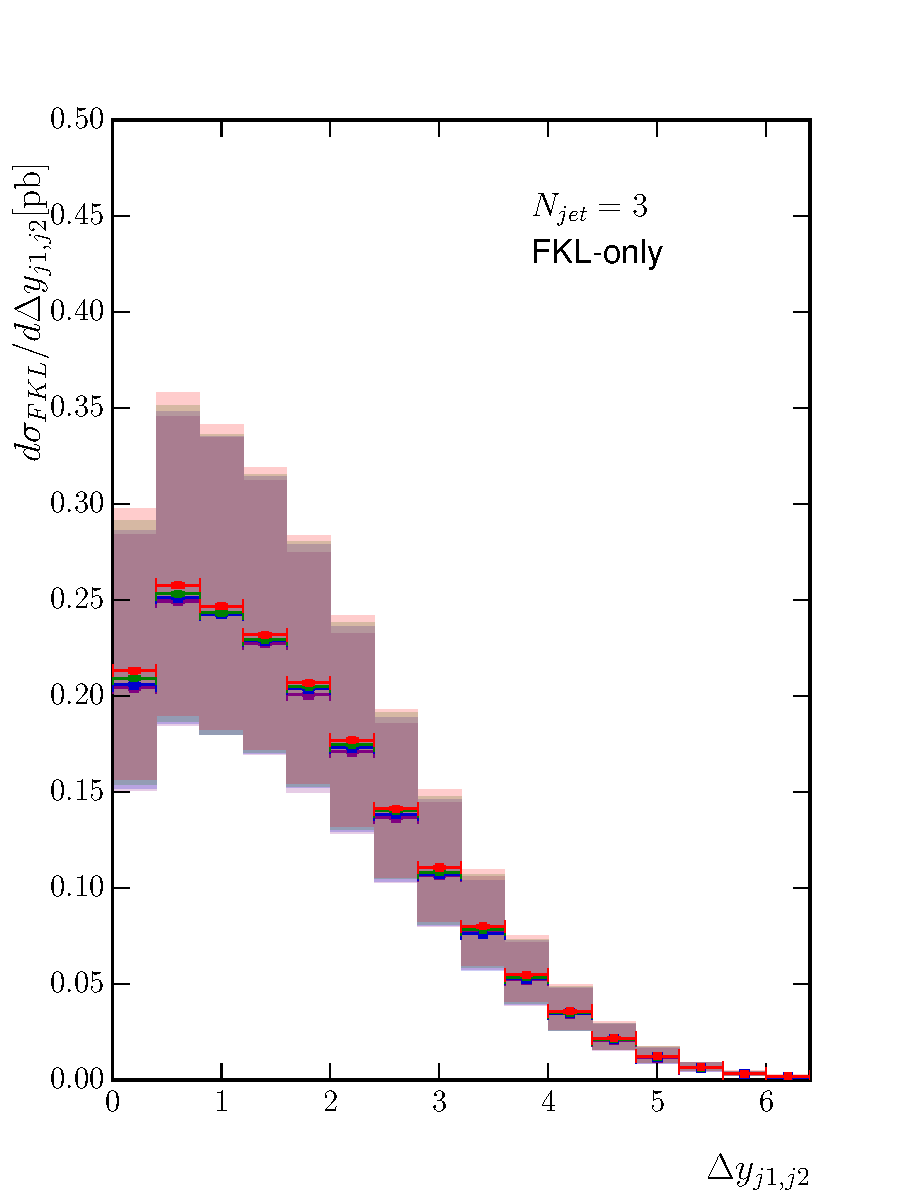
\includegraphics[width=.5\textwidth]{Z_11a_3j.pdf}\hfill
		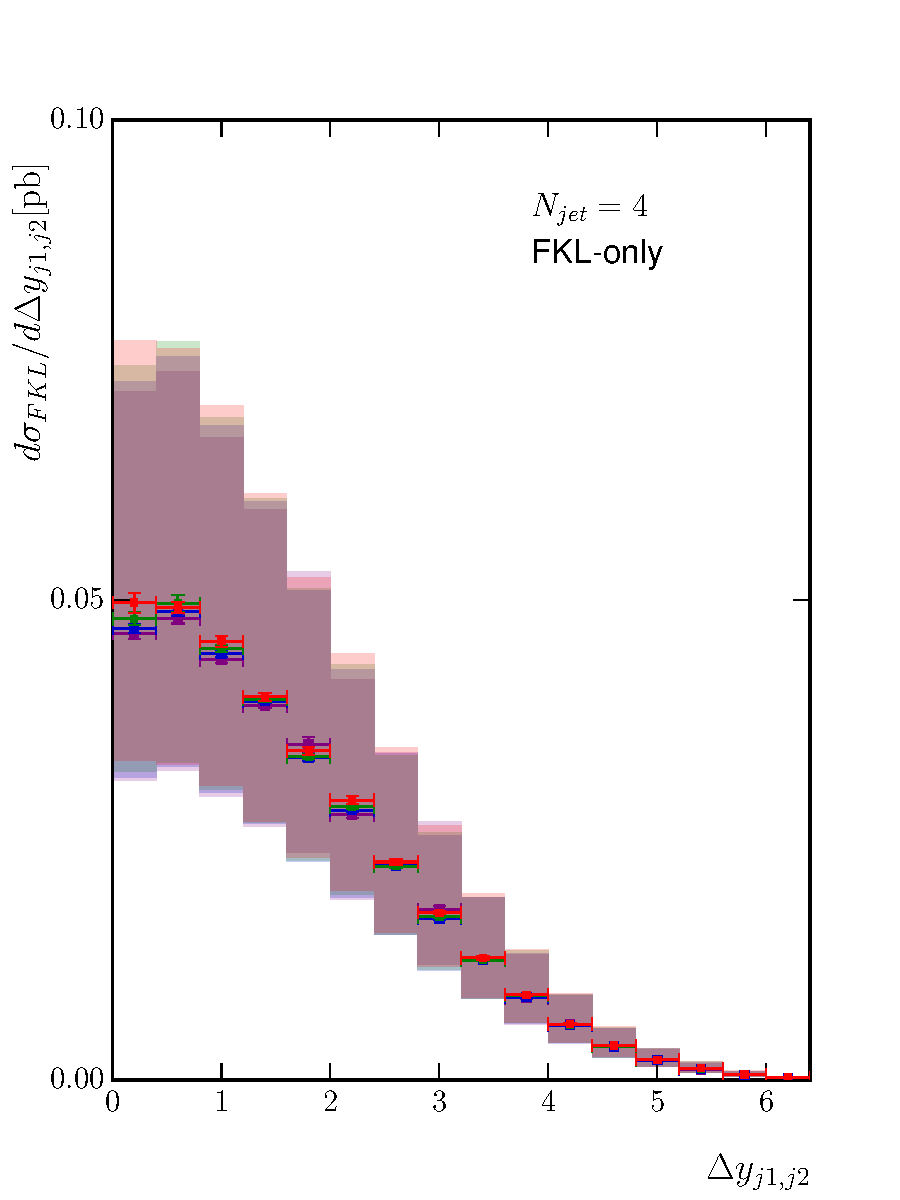
\includegraphics[width=.5\textwidth]{Z_11a_4j.pdf}
		\caption{The effect of varying $\lambda_{cut}$ on the differential distribution
		in the rapidity gap between the two leading jets in $p_\perp$, $\Delta y_{j1, j2}$, with the $N_{jet}=2,3,4$
		exclusive selections shown from left to right.  $\lambda_{cut}=0.2$ (red), 0.5 (blue), 1.0 (green), 2.0 (purple).}
		\label{fig:lambdadist}
	\end{figure}

	\begin{figure}[htp!]
		\centering
		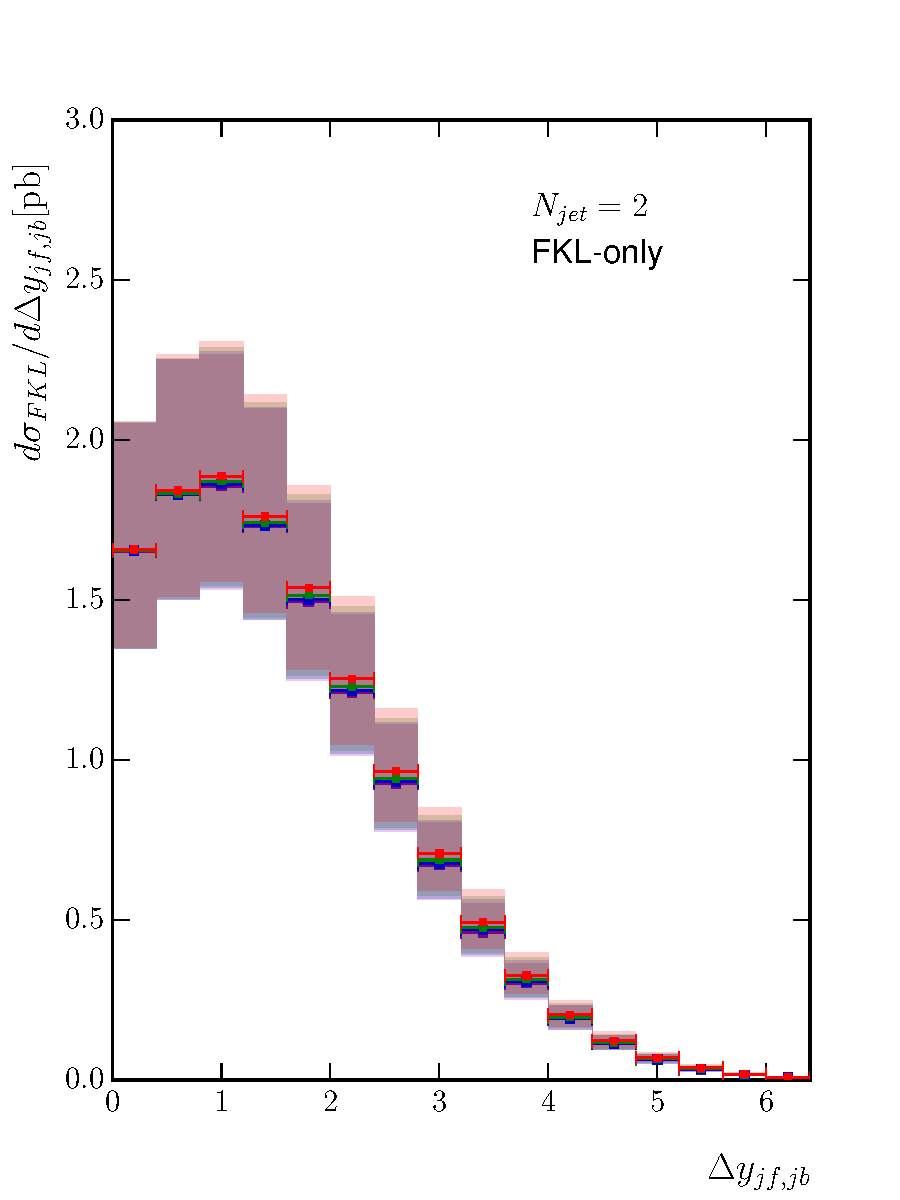
\includegraphics[width=.5\textwidth]{Z_11c_2j.pdf}\hfill
		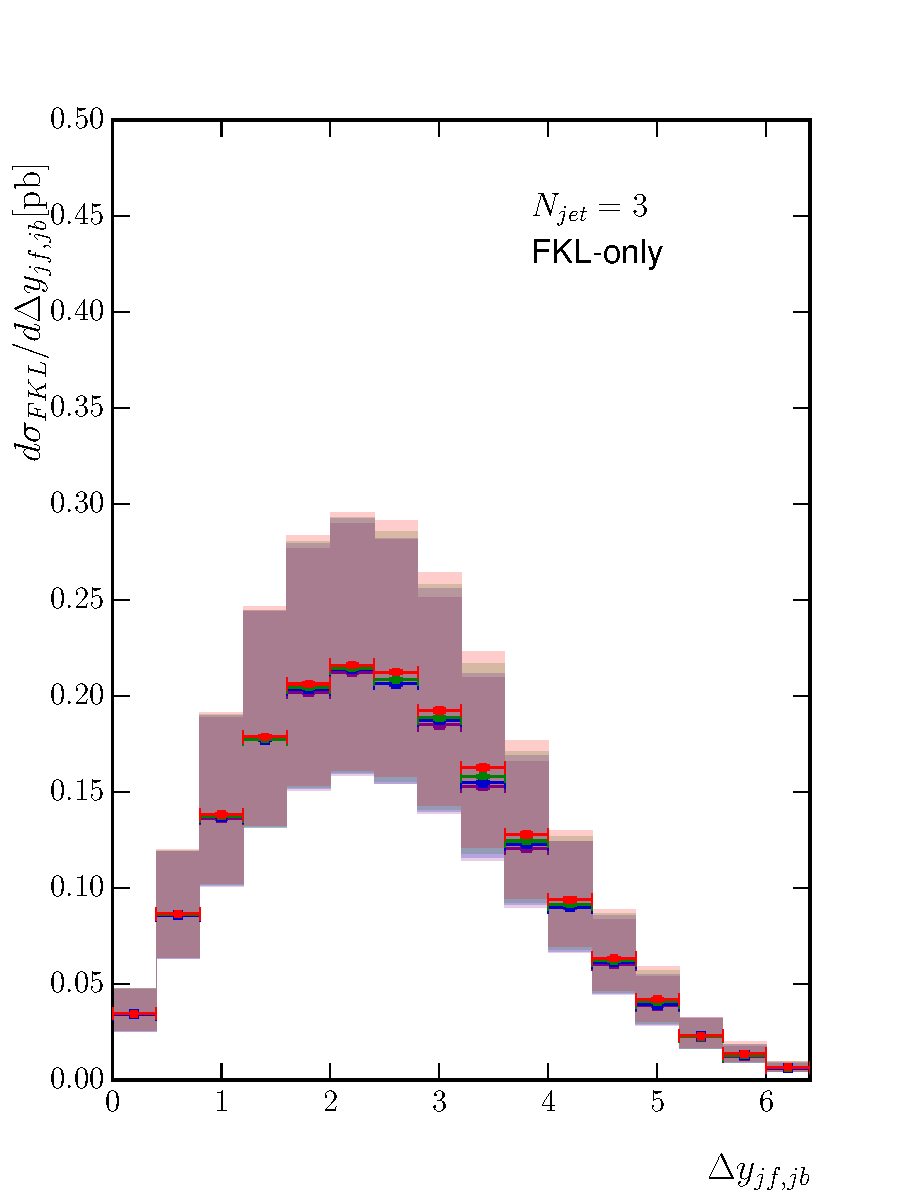
\includegraphics[width=.5\textwidth]{Z_11c_3j.pdf}\hfill
		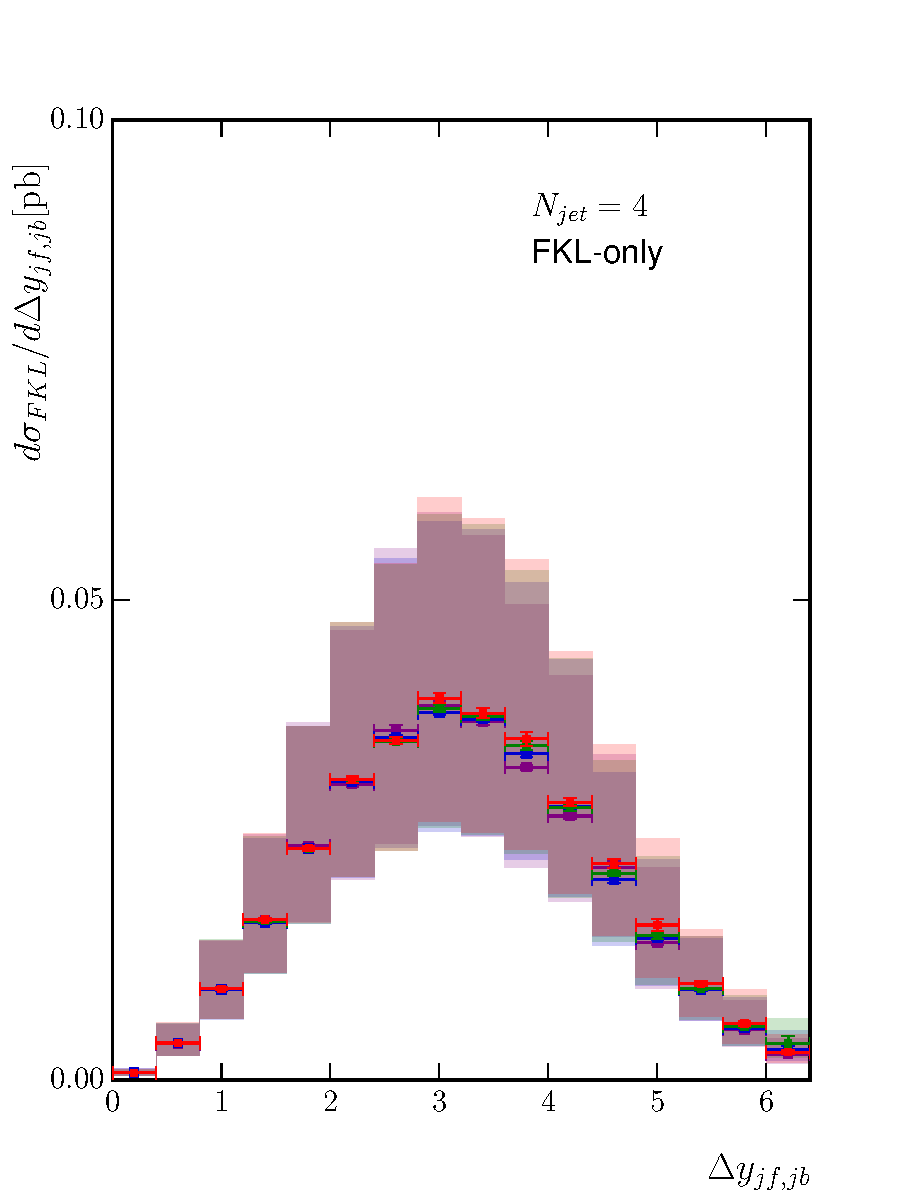
\includegraphics[width=.5\textwidth]{Z_11c_4j.pdf}
		\caption{The effect of varying $\lambda_{cut}$ on the differential distribution
		in the rapidity gap between the two extremal jets in rapidity, $\Delta y_{jf, jb}$, with the $N_{jet}=2,3,4$
		exclusive selections shown from left to right.  $\lambda_{cut}=0.2$ (red), 0.5 (blue), 1.0 (green), 2.0 (purple).}
		\label{fig:lambdadistdy}
	\end{figure}

\section{$\zg$+Jets: Computational Aspects}

	\begin{itemize}
		\item Chat about the coding that went in to it
		\item Interference and scale variation in the Z's
		\item Q-chains/V-chains
		\item Complicated currents
		\item GRID stuff?
	\end{itemize}

\section{$\zg$+Jets at the LHC}

	\subsection{$\zg$+Jets at the ATLAS Experiment}

		\begin{itemize}
			\item Re-word descriptions of plots
		\end{itemize}

		We now compare the results of the formalism described in the previous sections
		to data.  We begin with a recent ATLAS analysis of $Z$-plus-jets events from
		7~TeV collisions~\cite{Aad:2013ysa}.  We summarise the cuts in the following
		table:

		\begin{table}[bth]
		  \centering
		  \begin{tabular}{|l|c|}
		    \hline
		    Lepton Cuts & $p_{T\ell}>20$~GeV, \; $|\eta_\ell|<2.5$ \\
		    & $\Delta R^{\ell^+\ell^-} > 0.2$, \; $66$~GeV $\leq m^{\ell^+\ell^-} \leq
		      116$~GeV \\ \hline
		    Jet Cuts (anti-$k_T$, 0.4) & $p_{Tj}>30$~GeV, \; $|y_j|<4.4$ \\
		    & $\Delta R^{j\ell} >0.5$ \\
		\hline
		  \end{tabular}
		  \caption{Cuts applied to theory simulations in the ATLAS
		    $Z$-plus-jets analysis results shown in Figs.~\ref{fig:ATLAS_2a}--\ref{fig:ATLAS_7b}.}
		  \label{tab:atlascuts}
		\end{table}

		Any jet which failed the final isolation cut was removed from the event, but the
		event itself is kept provided there are a sufficient number of other jets
		present.  Throughout the central value of the HEJ predictions has been
		calculated with factorisation and renormalisation scales set to
		$\mu_F=\mu_R=H_T/2$, and the theoretical uncertainty band has been determined by
		varying these independently by up to a factor of 2 in each direction (removing
		the corners where the relative ratio is greater than two).  Also shown in the
		plots taken from the ATLAS paper are theory predictions from
		Alpgen~\cite{Mangano:2002ea}, Sherpa~\cite{Gleisberg:2008ta,Hoeche:2012yf},
		MC@NLO~\cite{Frixione:2002ik} and
		BlackHat+Sherpa~\cite{Berger:2010vm,Ita:2011wn}.  We will also comment on the
		recent theory description of Ref.\cite{Frederix:2015eii} .

		In Fig.~\ref{fig:ATLAS_2a}, we begin this set of comparisons with predictions
		and measurements of the inclusive jet rates.  HEJ and most of the other theory
		descriptions give a reasonable description of these rates.  The MC@NLO
		prediction drops below the data because it only contains the hard-scattering
		matrix element for $\zg$ production and relies on a parton shower for additional
		emissions. The HEJ predictions have a larger uncertainty band which largely
		arises from the use of leading-order results in the matching procedures.

		The first differential distribution we consider here is the distribution of the
		invariant mass between the two hardest jets, Fig.~\ref{fig:ATLAS_11b}.  The
		region of large invariant mass is particularly important because this is a
		critical region for studies of vector boson fusion (VBF) processes in
		Higgs-plus-dijets.  Radiation patterns are largely universal between these
		processes, so one can test the quality of theoretical descriptions in
		$\zg$-plus-dijets and use these to inform the VBF analyses.  It is also a
		distribution which will be studied to try to detect subtle signs of new physics.
		In this study, HEJ and the other theory descriptions all give a good description
		of this variable out to 1~TeV, with HEJ being closest throughout the range.  The
		merged sample of Ref.~\cite{Frederix:2015eii} (Fig.~9 in that paper) combined
		with the Pythia8 parton shower performs reasonably well throughout the range
		with a few deviations of more than 20\%, while that combined with Herwig++
		deviates badly.  In a recent ATLAS analysis of $W$-plus-dijet
		events~\cite{Aad:2014qxa}, the equivalent distribution was extended out to 2~TeV
		and almost all of the theoretical predictions deviated significantly while the
		HEJ prediction remained flat.  This is one region where the high-energy
		logarithms which are only included in HEJ are expected to become large.

		In Fig.~\ref{fig:ATLAS_11a}, we show the comparison of various theoretical
		predictions to the distribution of the absolute rapidity difference between the
		two leading jets.  It is clear in the left plot that HEJ gives an excellent
		description of this distribution.  This is to some extent expected as
		high-energy logarithms are associated with rapidity separations.  However, this
		variable is only the rapidity separation between the two hardest jets which is
		often not representative of the event as harder jets tend to be more central.
		Nonetheless, the HEJ description performs well in this restricted scenario.  The
		next-to-leading order (NLO) calculation of Blackhat+Sherpa also describes the
		distribution quite well while the other merged, fixed-order samples deviate from
		the data at larger values.  The merged samples of Ref.~\cite{Frederix:2015eii}
		(Fig.~8 in that paper) describe this distribution well for small values of this
		variable up to about 3 units when combined with Herwig++ and for most of the
		range when combined with the Pythia8 parton shower, only deviating above 5 units.

		The final distribution in this section is that of the ratio of the transverse
		momentum of the second hardest jet to the hardest jet.  The perturbative
		description of HEJ does not contain any systematic evolution of transverse
		momentum and this can be seen where its prediction undershoots the data at low
		values of $p_{T2}/p_{T1}$.  However, for values of $p_{T2} \gtrsim 0.5 p_{T1}$,
		the ratio of the HEJ prediction to data is extremely close to 1.  The
		fixed-order based predictions shown in Fig.~\ref{fig:ATLAS_2a} are all fairly
		flat above about 0.2, but the ratio of the data differs by about 10\%.

		\newpage

		\begin{figure}[H]
		  \centering
		  \begin{subfigure}[b]{0.48\textwidth}
		    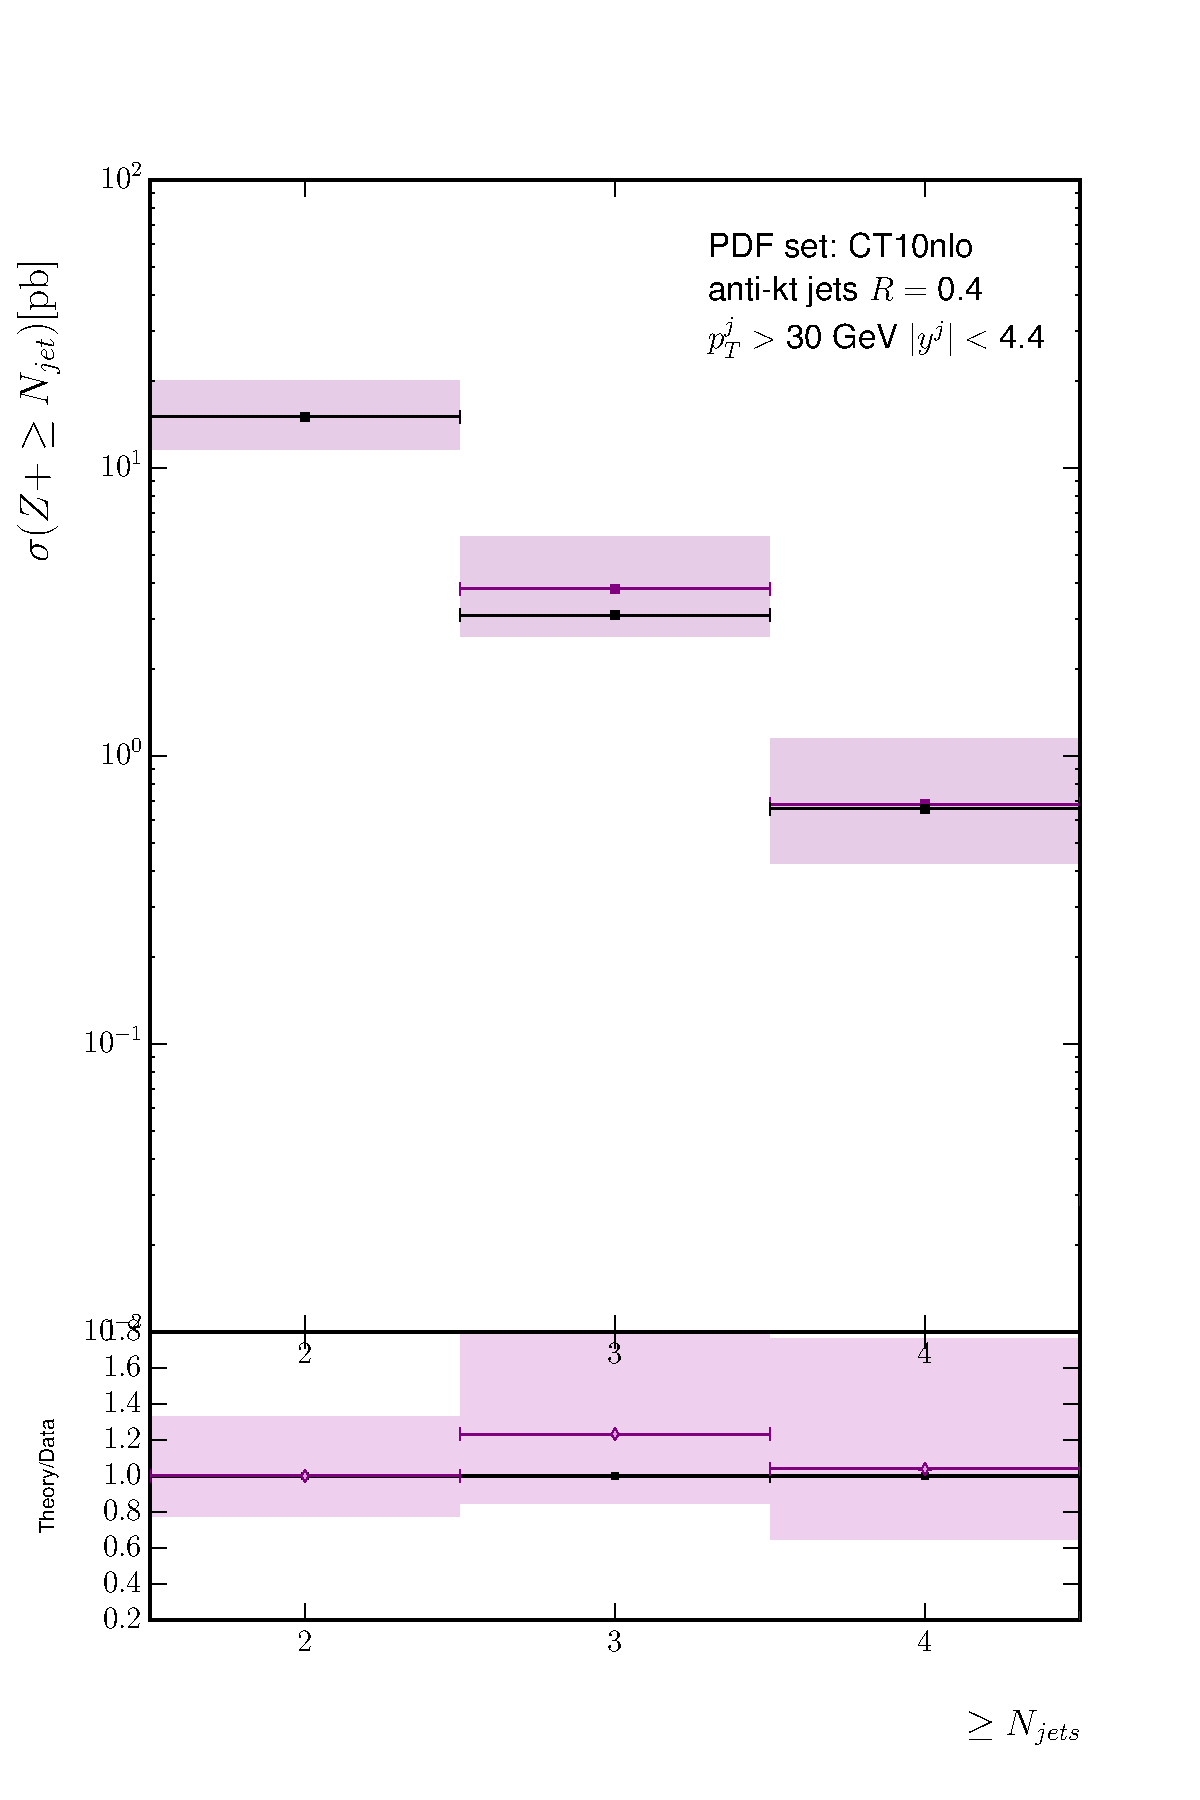
\includegraphics[width=\textwidth, height=1.2\textwidth]{ATLAS_Z_2a}
		    \label{fig:HEJ_ATLAS_2a}
		  \end{subfigure}
		  ~
		  \begin{subfigure}[b]{0.48\textwidth}
		    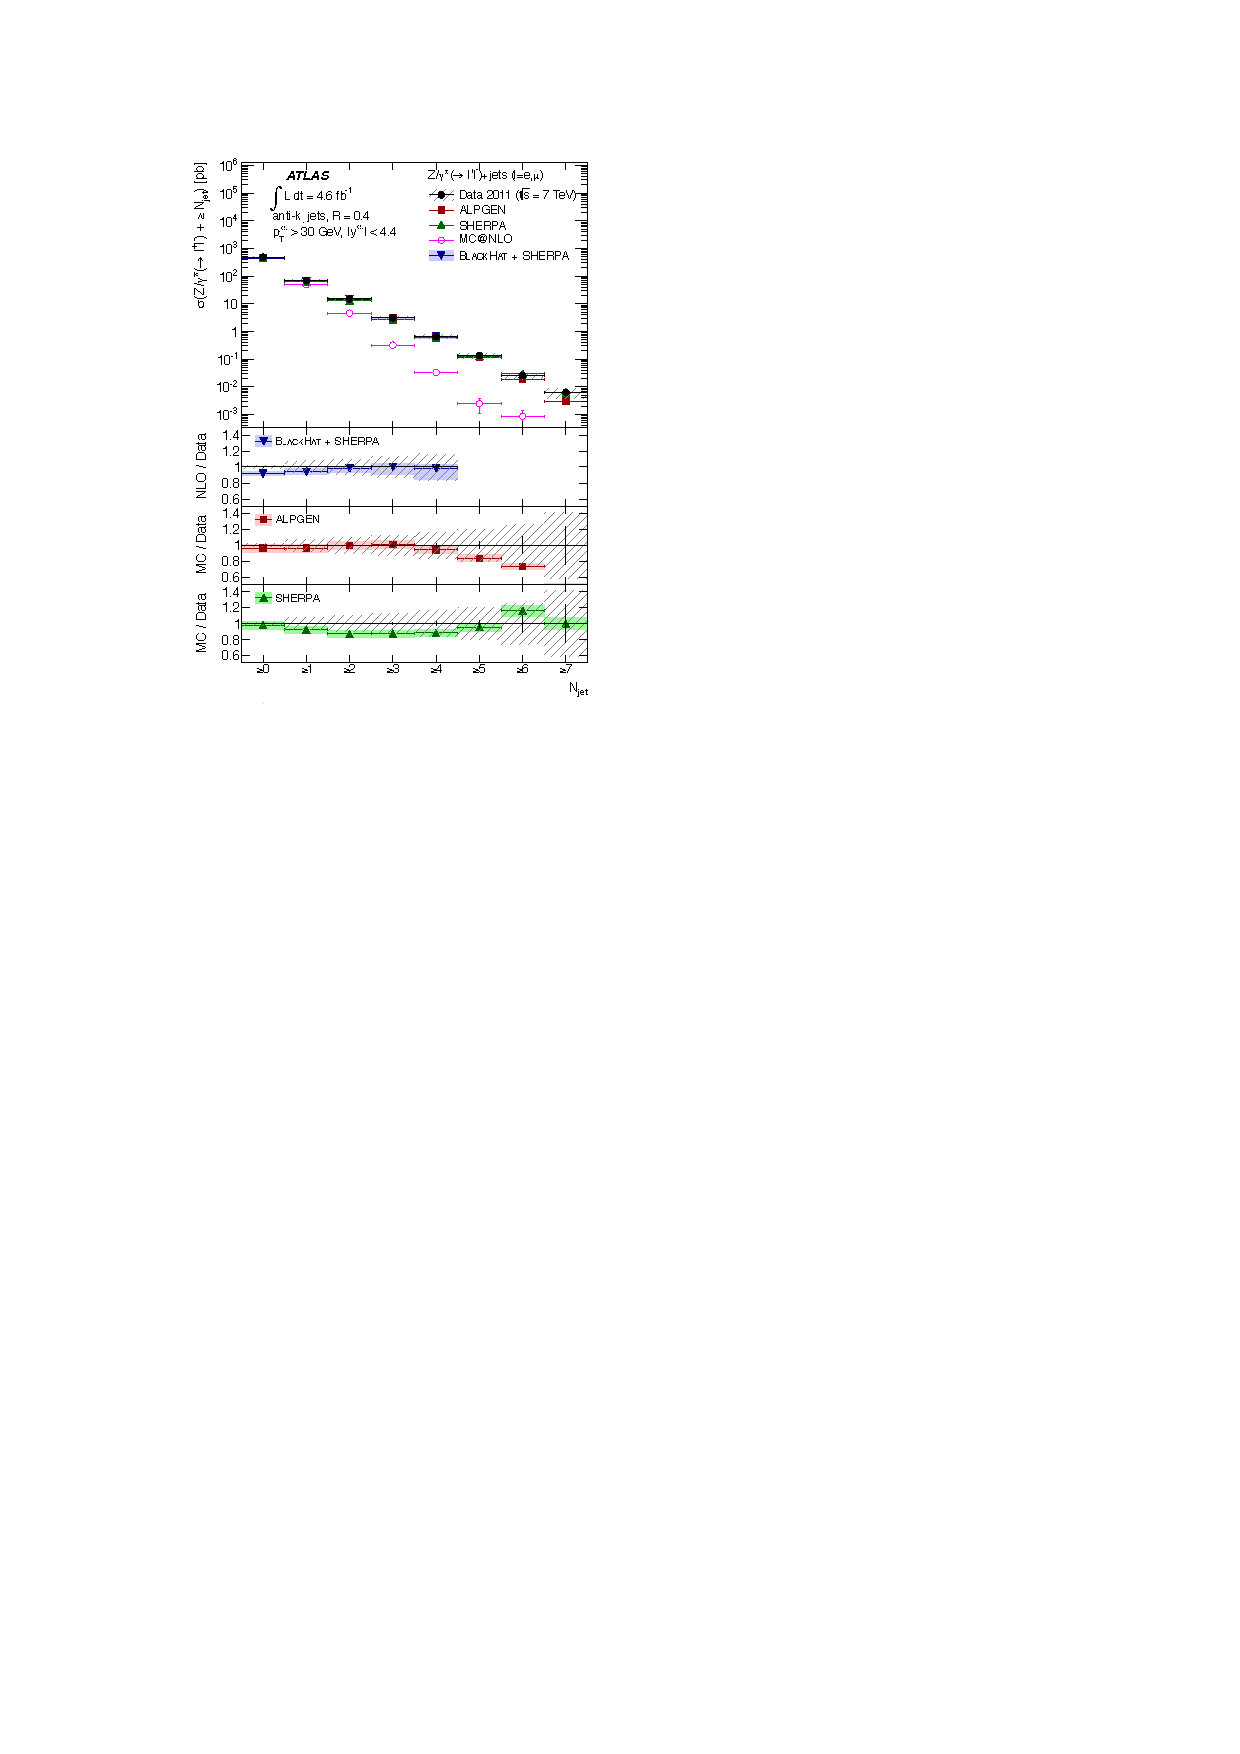
\includegraphics[width=\textwidth, height=1.2\textwidth]{Comparison_2a}
		    \caption{}
		    \label{fig:MC_ATLAS_2a}
		  \end{subfigure}
		  \caption{These plots show the inclusive jet rates from (a) HEJ and (b) other
		    theory descriptions and data~\cite{Aad:2013ysa}.  HEJ events all contain at
		    least two jets and do not contain matching for 5 jets and above, so these
		    bins are not shown.}
		  \label{fig:ATLAS_2a}

		  \begin{subfigure}[b]{0.48\textwidth}
		    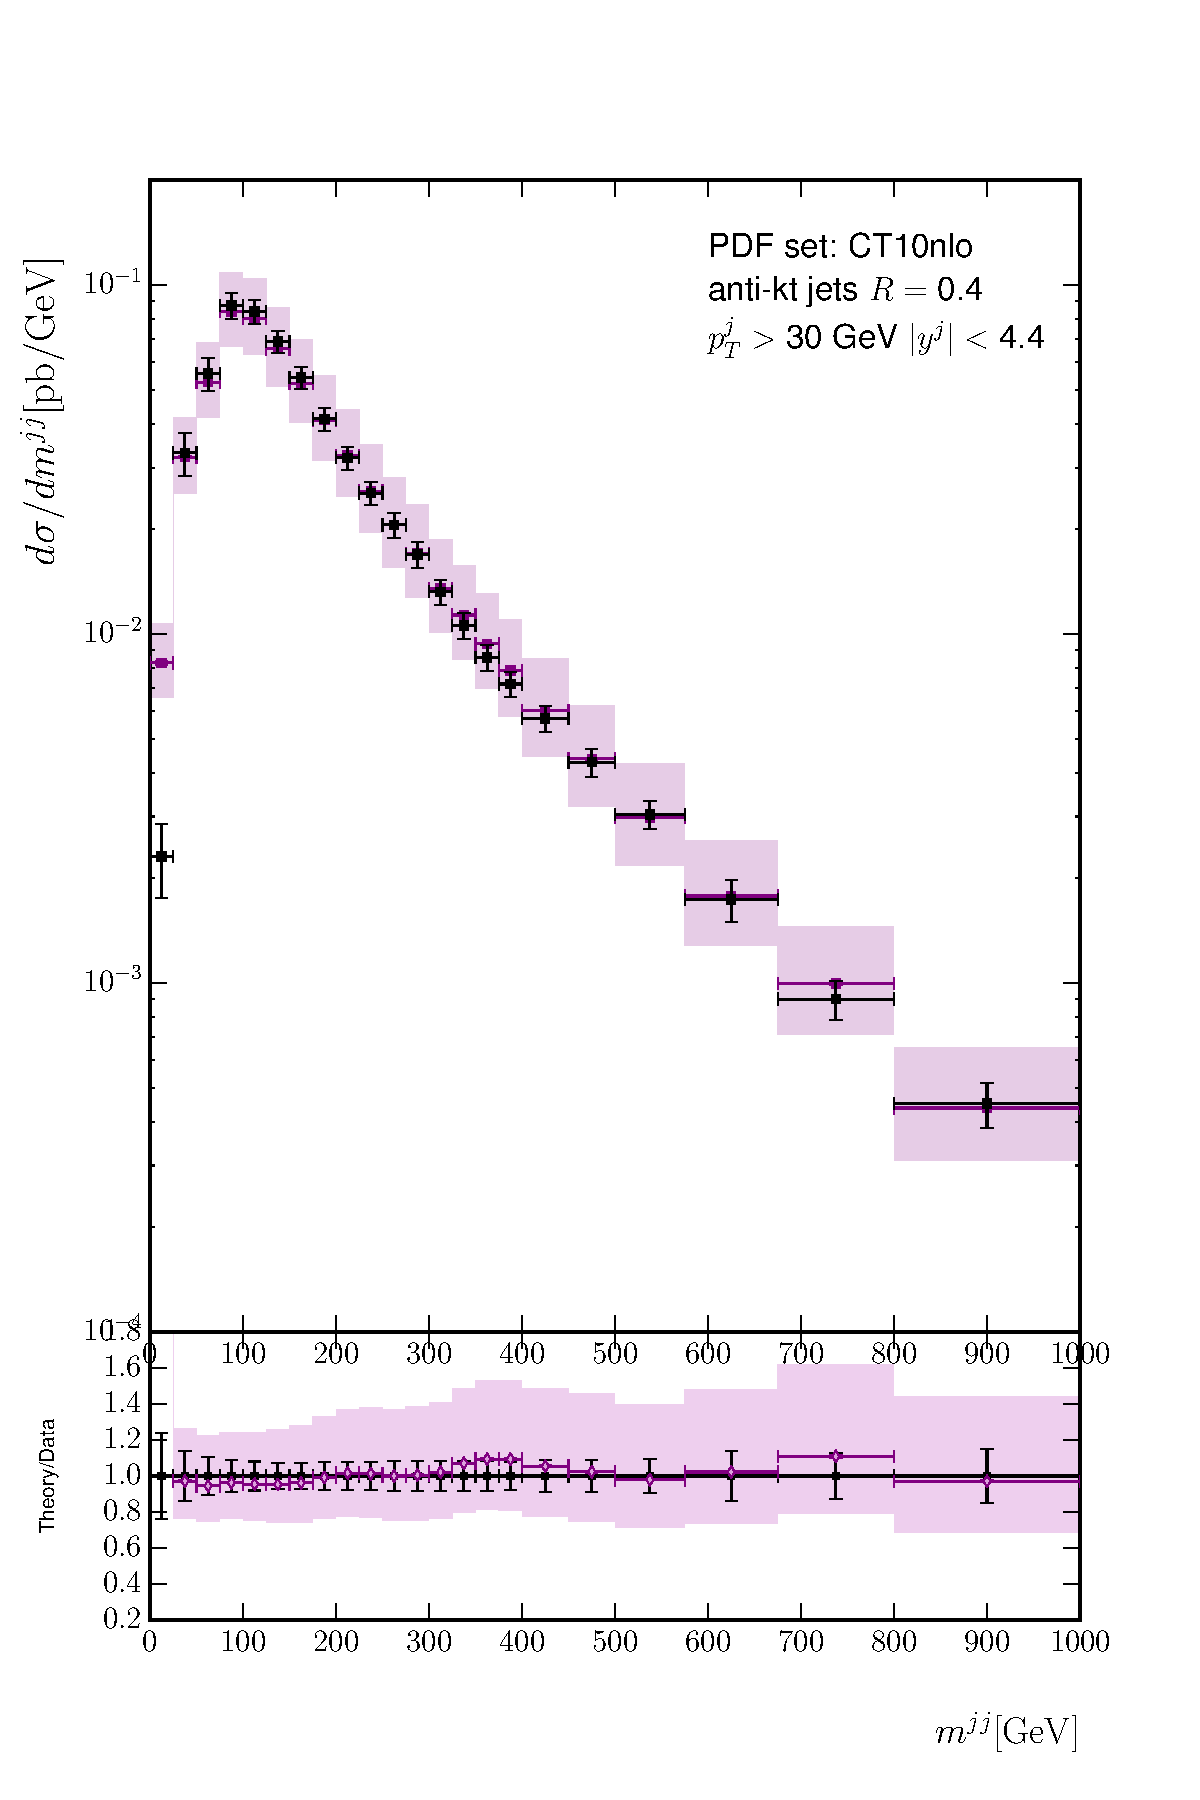
\includegraphics[width=\textwidth, height=1.2\textwidth]{ATLAS_Z_11b}
		    \caption{}
		    \label{fig:HEJ_ATLAS_11b}
		  \end{subfigure}
		  ~
		  \begin{subfigure}[b]{0.48\textwidth}
		    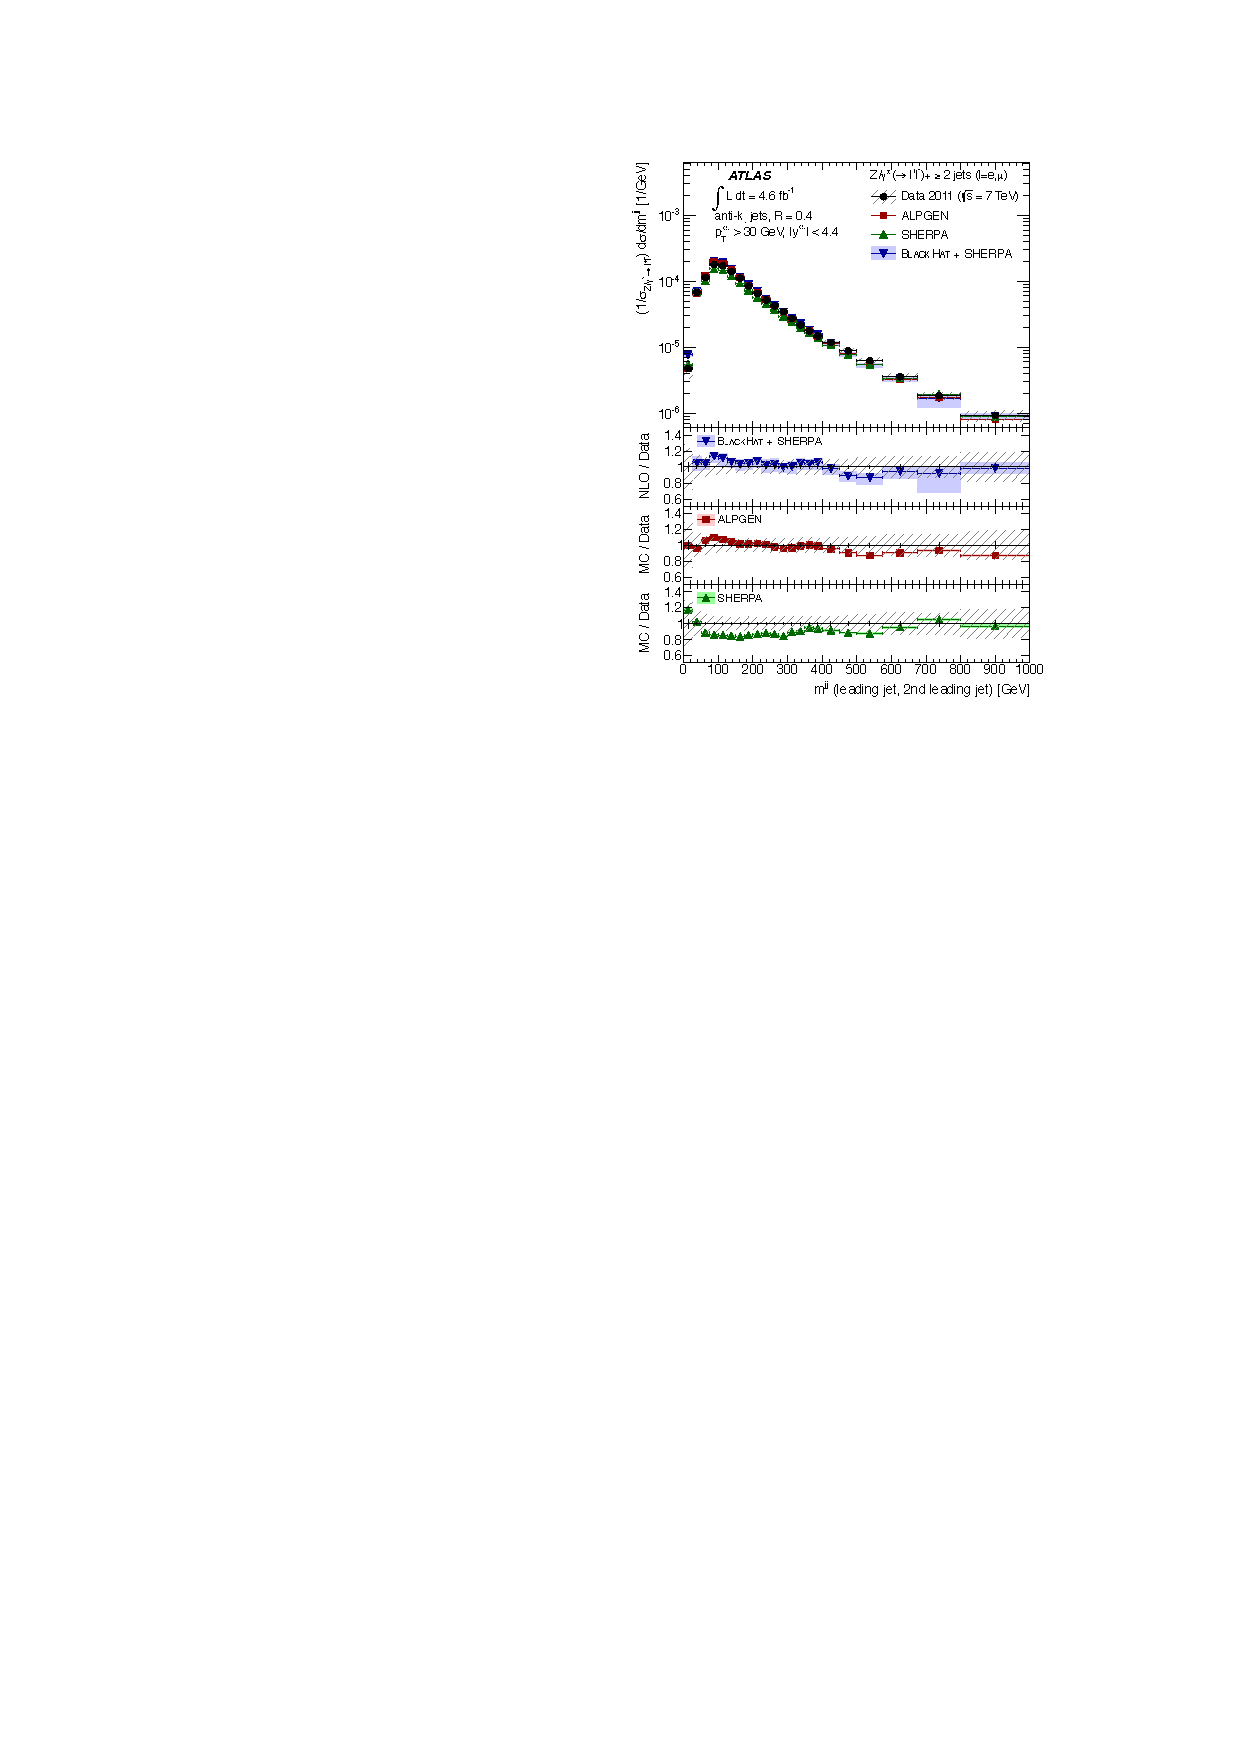
\includegraphics[width=\textwidth, height=1.2\textwidth]{Comparison_11b}
		    \caption{}
		    \label{fig:MC_ATLAS_11b}
		  \end{subfigure}
		  \caption{These plots show the invariant mass between the leading and
		    second-leading jet in $p_T$.  As in Fig.~\ref{fig:ATLAS_2a}, predictions are
		    shown from (a) HEJ and (b) other theory descriptions and
		    data~\cite{Aad:2013ysa}. These studies will inform Higgs plus dijets
		    analyses, where cuts are usually applied to select events with large
		    $m_{12}$.}
		  \label{fig:ATLAS_11b}
		\end{figure}

		\begin{figure}[h]
		  \centering
		  \begin{subfigure}[b]{0.48\textwidth}
		    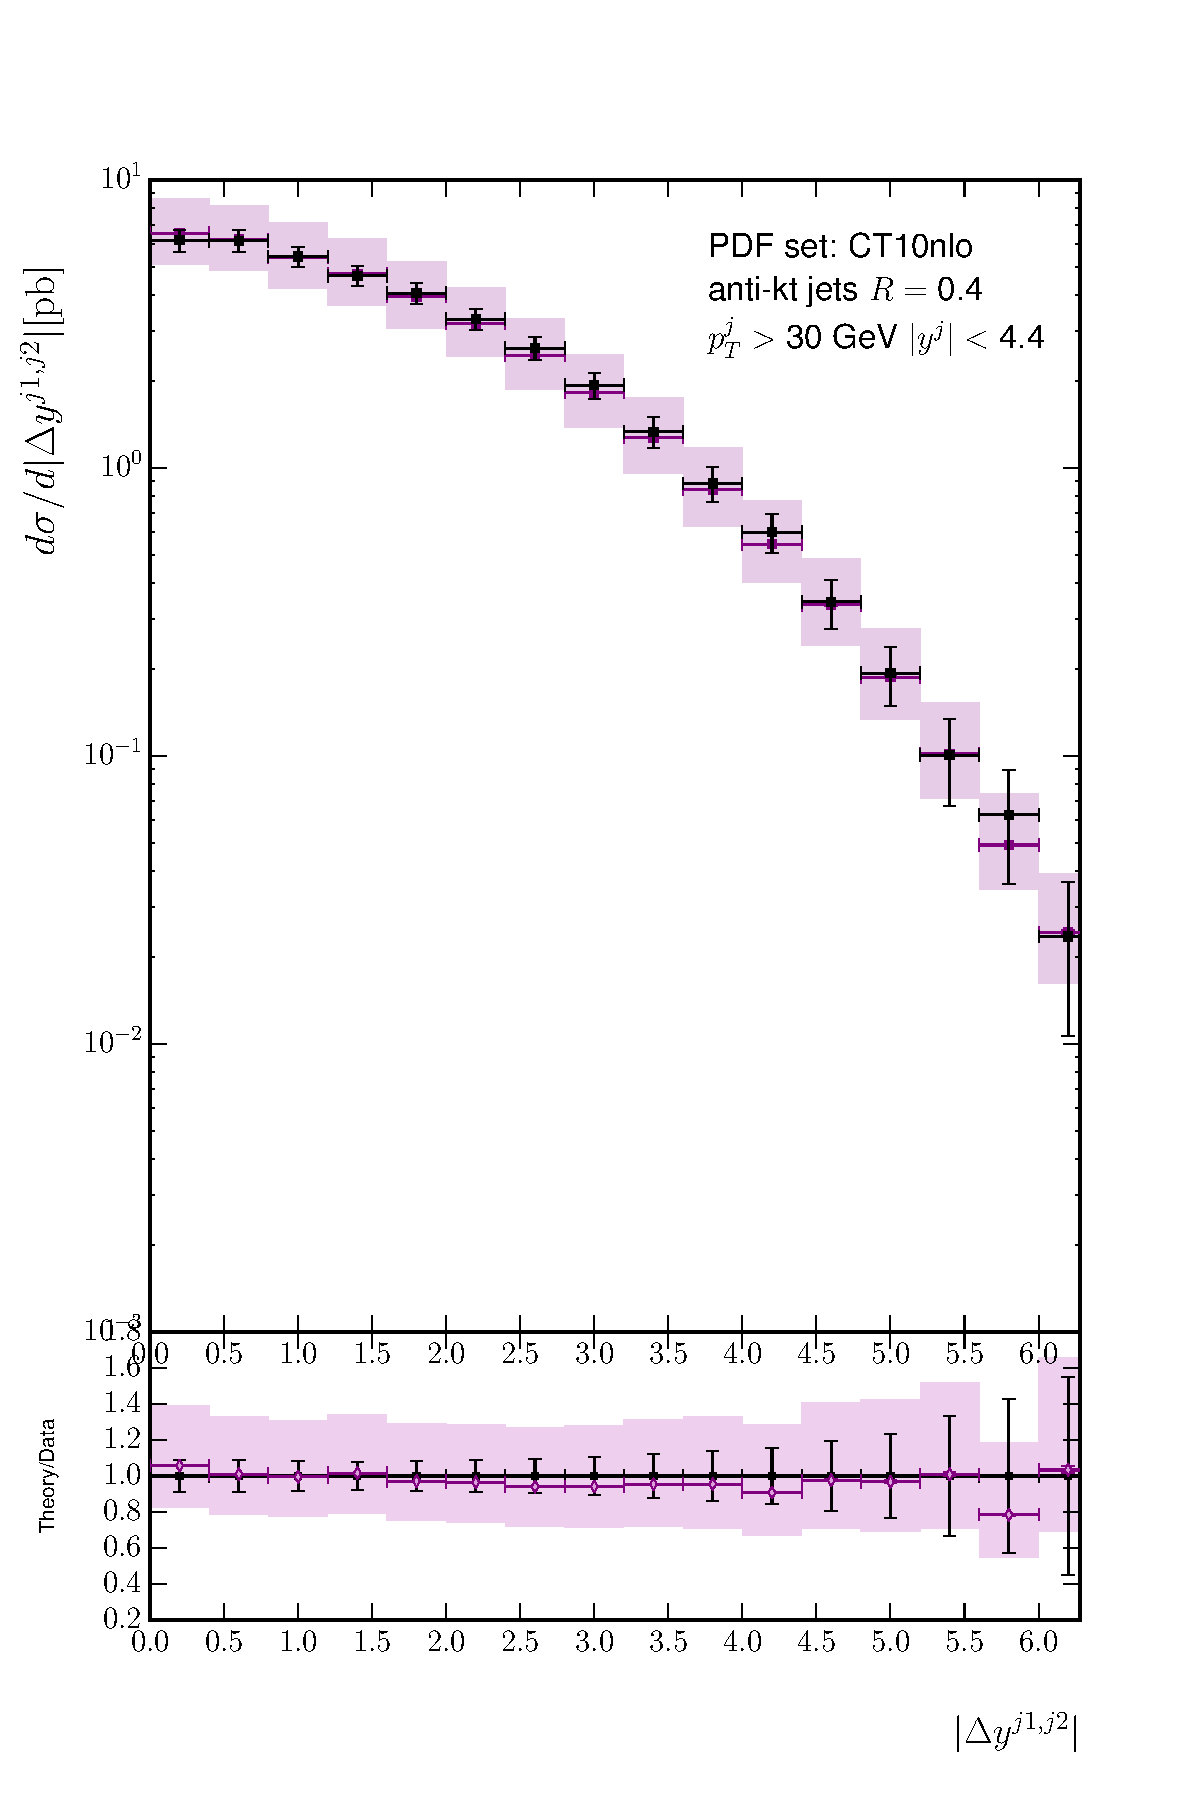
\includegraphics[width=\textwidth, height=1.2\textwidth]{ATLAS_Z_11a}
		    \caption{}
		    \label{fig:HEJ_ATLAS_11a}
		  \end{subfigure}
		  ~
		  \begin{subfigure}[b]{0.48\textwidth}
		    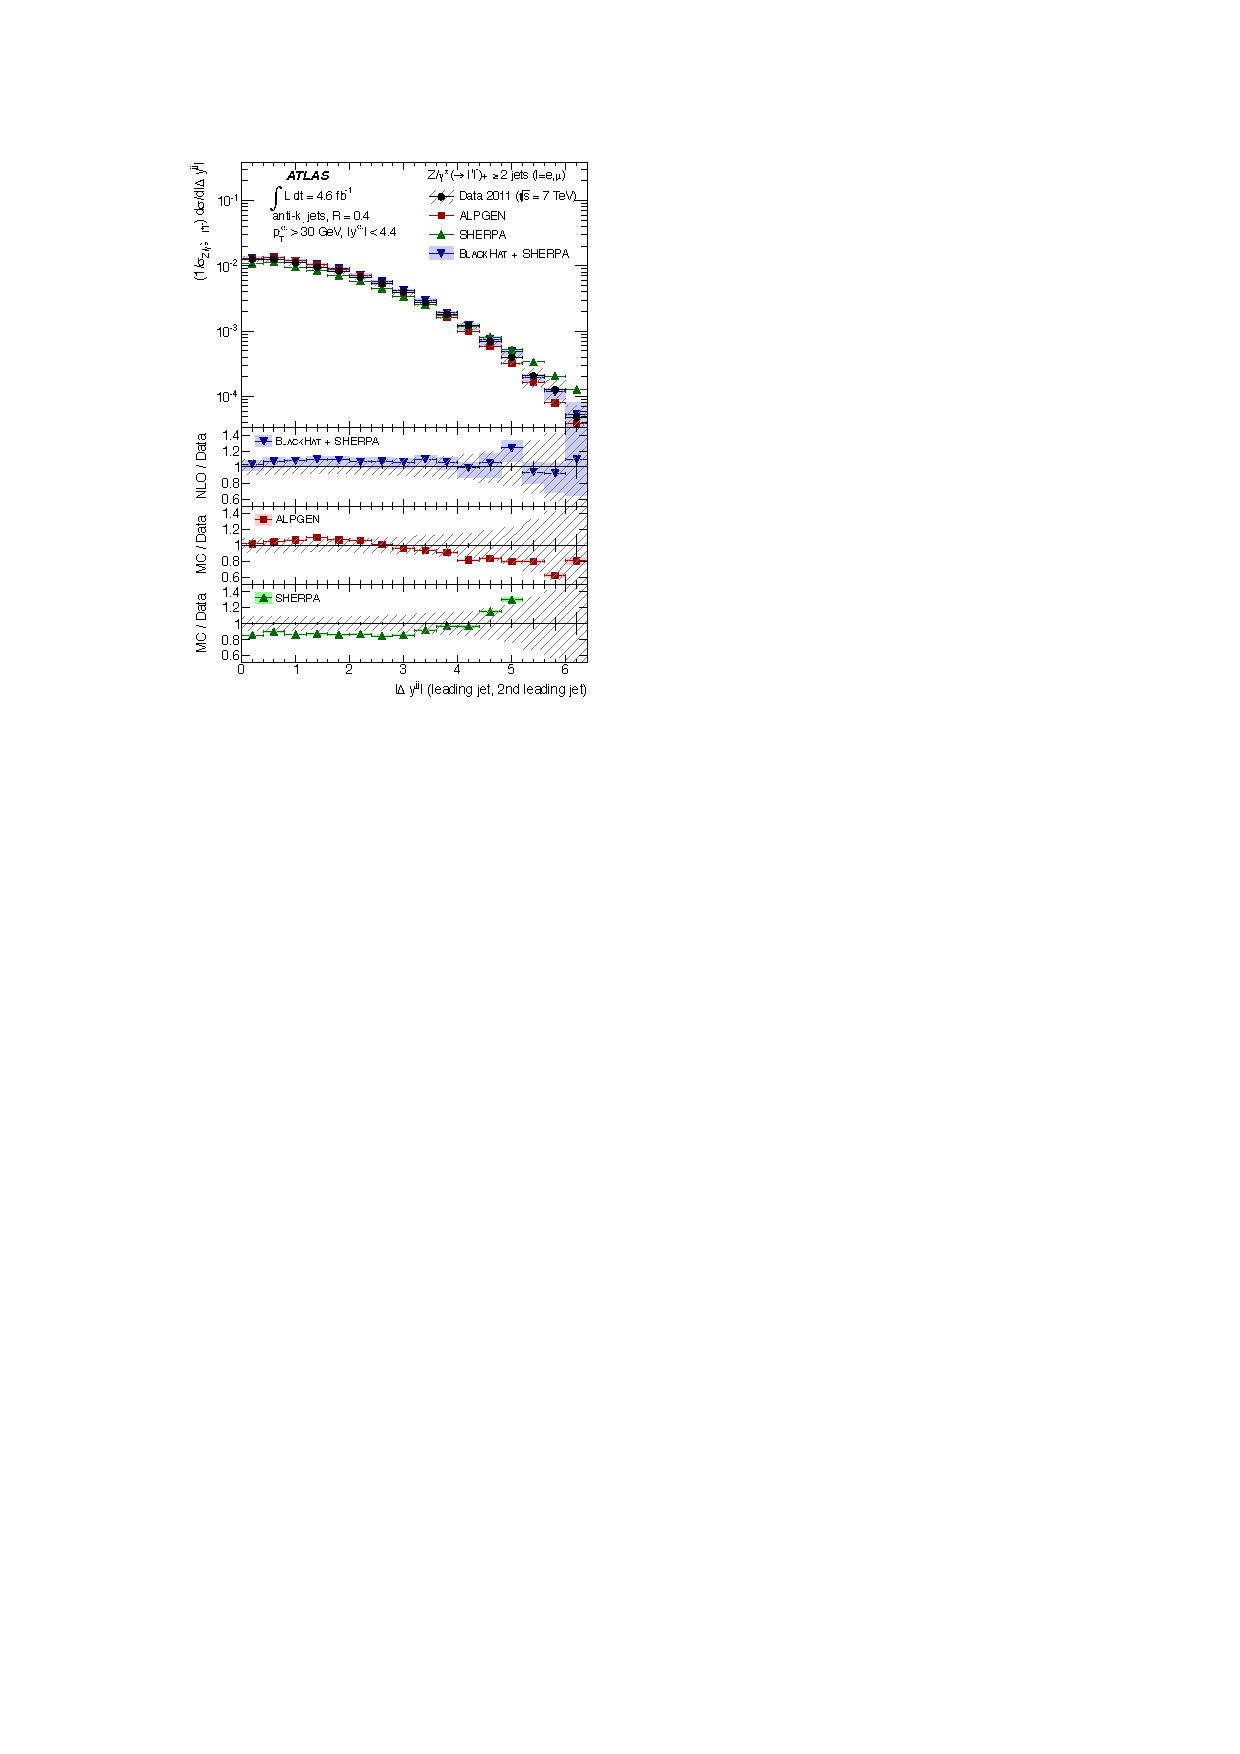
\includegraphics[width=\textwidth, height=1.2\textwidth]{Comparison_11a}
		    \caption{}
		    \label{fig:MC_ATLAS_11a}
		  \end{subfigure}
		  \caption{The comparison of (a) HEJ and (b) other theoretical descriptions and
		    data~\cite{Aad:2013ysa} to
		    the distribution of the absolute rapidity different between the two leading
		    jets.  HEJ and Blackhat+Sherpa give the best description.}
		  \label{fig:ATLAS_11a}

		  \begin{subfigure}[b]{0.48\textwidth}
		    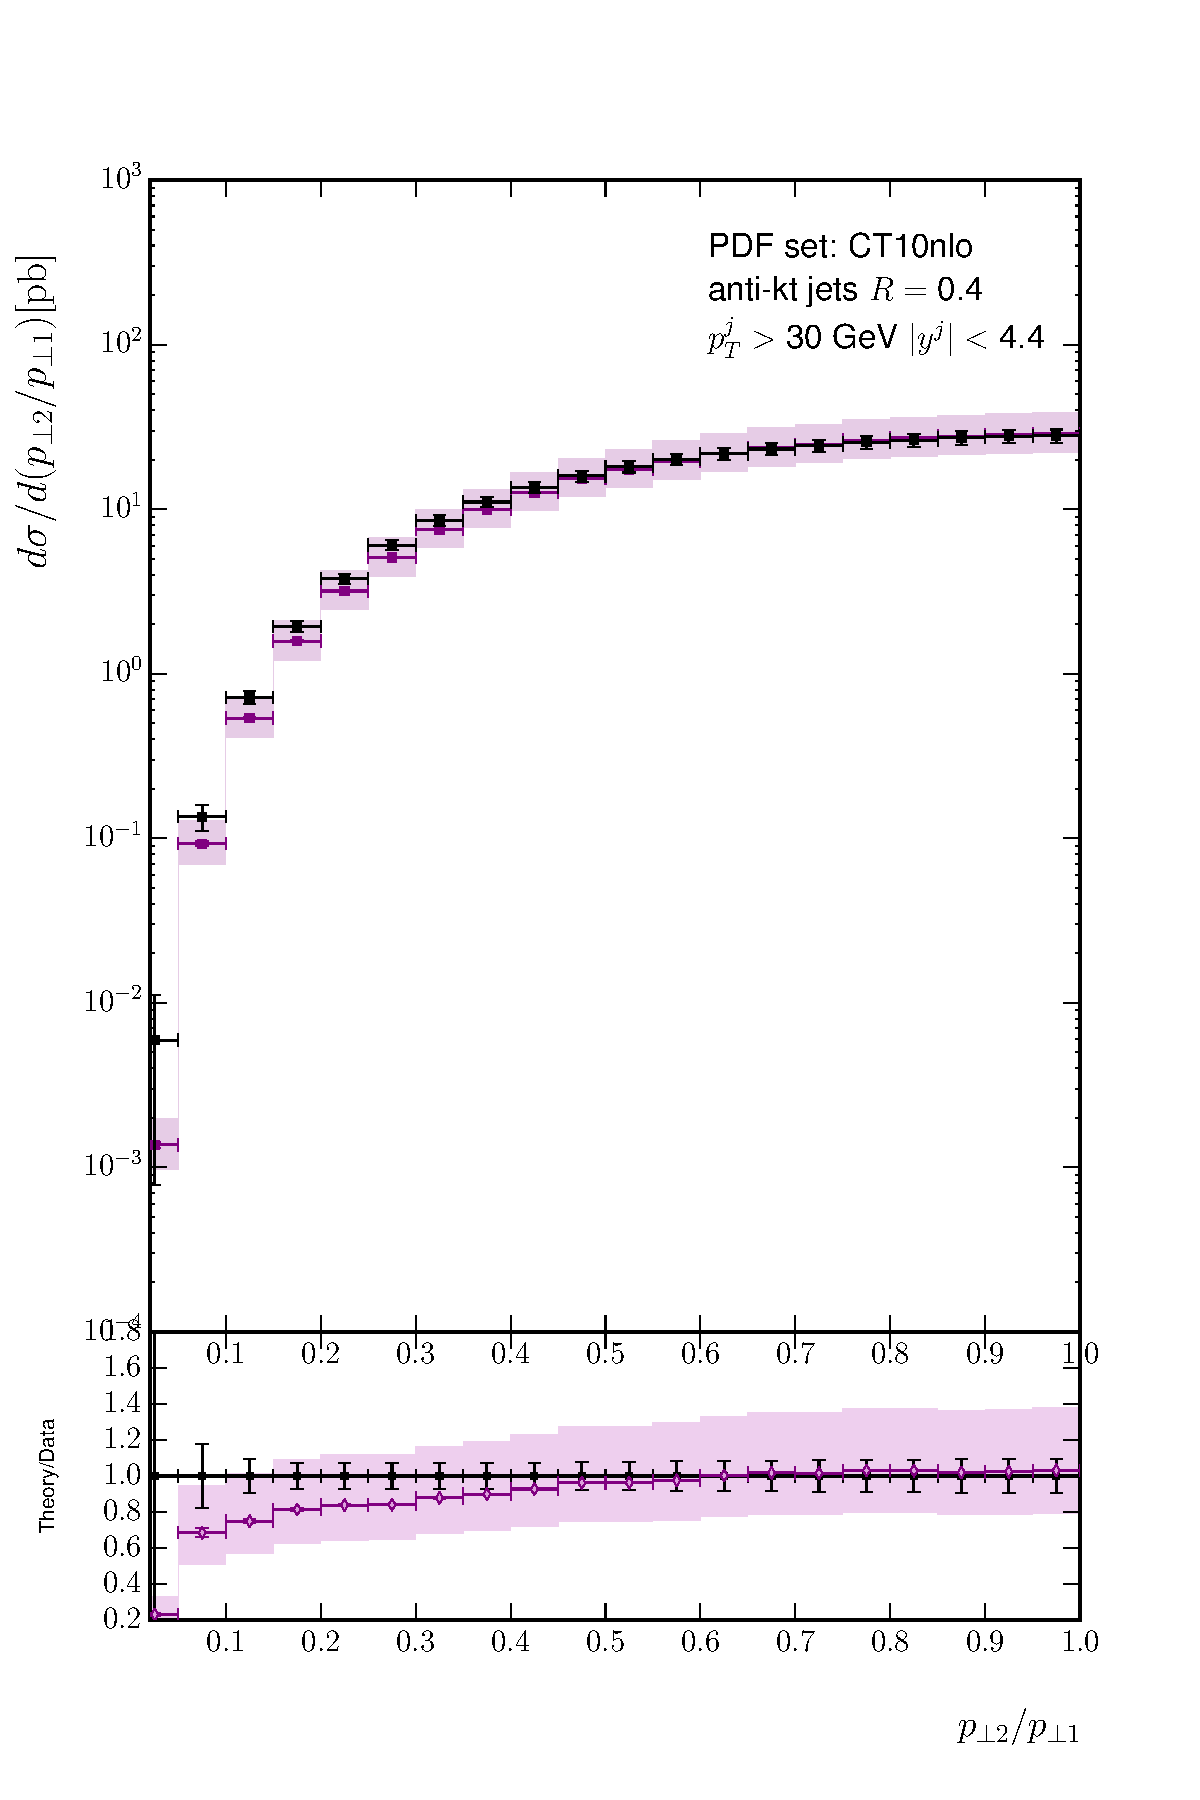
\includegraphics[width=\textwidth, height=1.2\textwidth]{ATLAS_Z_7b}
		    \caption{}
		    \label{fig:HEJ_ATLAS_7b}
		  \end{subfigure}
		  ~
		  \begin{subfigure}[b]{0.48\textwidth}
		    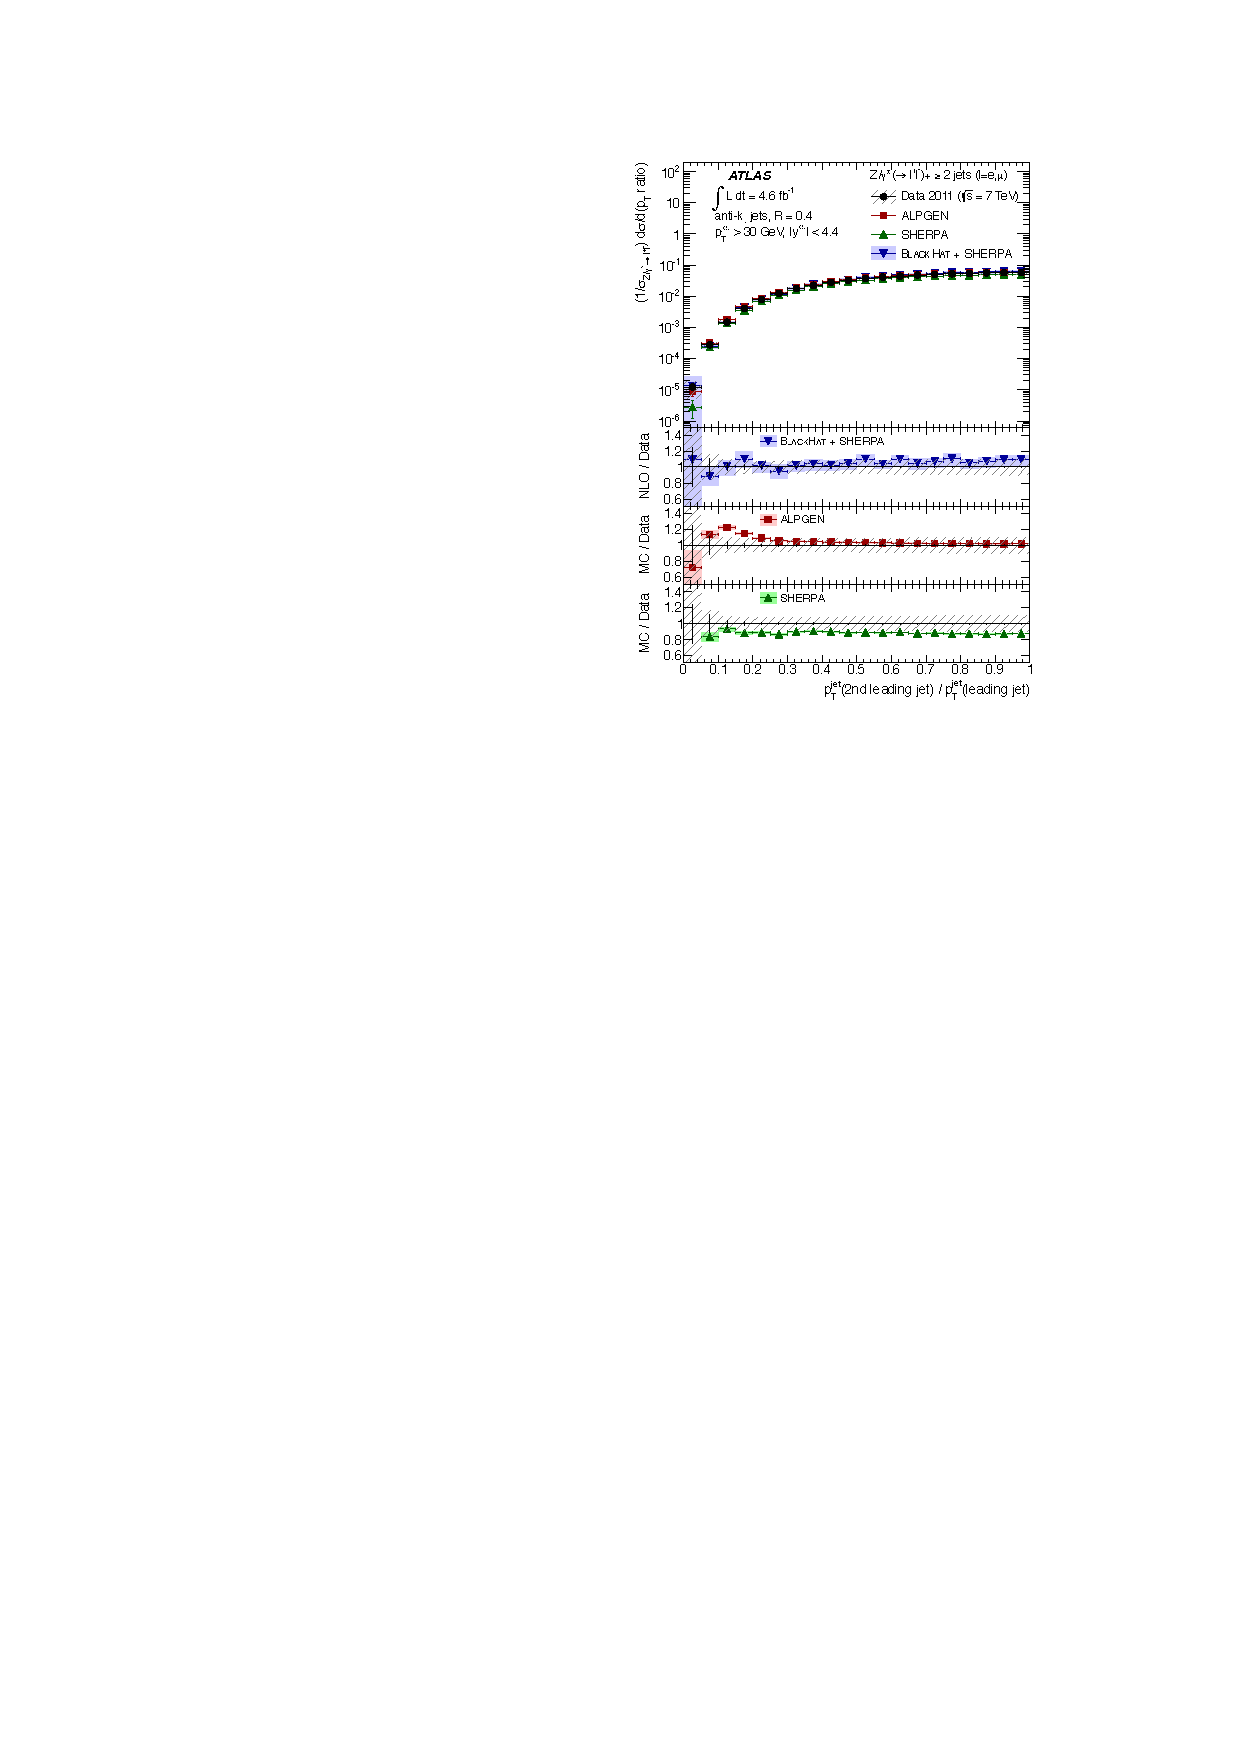
\includegraphics[width=\textwidth, height=1.2\textwidth]{Comparison_7b}
		    \caption{}
		    \label{fig:MC_ATLAS_7b}
		  \end{subfigure}
		  \caption{These plots show the differential cross section in the ratio of the leading
		     and second leading jet in $p_T$ from (a) HEJ and (b) other
		    theory descriptions and data~\cite{Aad:2013ysa}.}
		  \label{fig:ATLAS_7b}
		\end{figure}

	\subsection{$\zg$+Jets at the CMS Experiment}
		\label{sub:CMS}

		We now compare to data from a CMS analysis of events with a $\zg$ boson produced
		in association with jets~\cite{Khachatryan:2014zya}.  We show, for comparison,
		the plots from that analysis which contain theoretical predictions from
		Sherpa~\cite{Gleisberg:2008ta,Hoeche:2012yf}, Powheg~\cite{Alioli:2010qp} and
		MadGraph~\cite{Alwall:2014hca}.The cuts used for this analysis are summarised in
		tab.~\ref{tab:cmscuts}.

		\begin{table}[hbt]
		  \centering
		  \begin{tabular}{|l|c|}
		    \hline
		    Lepton Cuts & $p_{T\ell}>20$~GeV, \; $|\eta_\ell|<2.4$ \\
		    &\; $71$~GeV $\leq m^{\ell^+\ell^-} \leq
		      111$~GeV \\ \hline
		    Jet Cuts (anti-$k_T$, 0.5) & $p_{Tj}>30$~GeV, \; $|y_j|<2.4$ \\
		    & $\Delta R^{j\ell} >0.5$ \\
		\hline
		  \end{tabular}
		  \caption{Cuts applied to theory simulations in the CMS
		    $Z$-plus-jets analysis results shown in
		    Figs.~\ref{fig:CMS_2a}--\ref{fig:CMS_3c}}
		  \label{tab:cmscuts}
		\end{table}

		As in the previous section, any jet which failed the final isolation cut was
		removed from the event, but the event itself is kept provided there are a
		sufficient number of other jets present.  The main difference to these cuts and
		those of ATLAS in the previous section is that the jets are required to be more
		central; $|\eta|<2.4$ as opposed to $|y|<4.4$.  This allows less room for
		evolution in rapidity; however, HEJ predictions are still relevant in this
		scenario.  Once again, the central values are given by $\mu_F=\mu_R=H_T/2$ with
		theoretical uncertainty bands determined by varying these independently by
		factors of two around this value.  HEJ events always contain a minimum of two
		jets and therefore here we only compare to the distributions for an event sample
		with at least two jets or above.

		We begin in Fig.~\ref{fig:CMS_2a} by showing the inclusive jet rates for these
		cuts.  The HEJ predictions give a good description, especially for the 2- and
		3-jet inclusive rates in this narrower phase space. The uncertainty bands are
		larger for HEJ than for the Sherpa and Powheg predictions due to our LO matching
		prescription (those for Madgraph are not shown).

		In Figs.~\ref{fig:CMS_3b}--~\ref{fig:CMS_3c}, we show the transverse momentum
		distributions for the second and third jet respectively (the leading jet
		distribution was not given for inclusive dijet events).  Beginning with the
		second jet in Fig.~\ref{fig:CMS_3b}, we see that the HEJ predictions overshoot
		the data at large transverse momentum.  In this region, the non-FKL matched
		components of the HEJ description become more important and these are not
		controlled by the high-energy resummation.  The HEJ predictions are broadly
		similar to Powheg's $Z$-plus-one-jet NLO calculation matched with the Pythia
		parton shower.  In contrast, Sherpa's prediction significantly undershoots the
		data at large transverse momentum.  Here the Madgraph prediction gives the best
		description of the data.

		% Fig.~\ref{fig:CMS_3c} shows the transverse momentum distribution of the third
		% jet in this data sample.  Here, the shape of HEJ prediction compared to the data
		% increases with transverse momentum, but the slope is not great and the deviation
		% is never greater than 20\%.  Both the Sherpa and Powheg predictions show greater
		% deviations.  This is not surprising for the Powheg prediction since it only
		% contains a hard-scattering matrix element for up to two jets.  The Madgraph
		% prediction again performs very well until the last bin.

		Fig.~\ref{fig:CMS_3c} shows the transverse momentum distribution of the third
		jet in this data sample.  Here, the ratio of the HEJ prediction to data shows a
		linear increase with transverse momentum (until the last bin where all the
		theory predictions show the same dip).  Both the Sherpa and Powheg predictions
		show similar deviations for this variable while the Madgraph prediction again
		performs very well.

		% Finally, we show the transverse momentum distribution of the fourth jet in
		% Fig.~\ref{fig:CMS_3d}.

		\begin{figure}[h]
		  \centering
		  \begin{subfigure}[b]{0.46\textwidth}
		    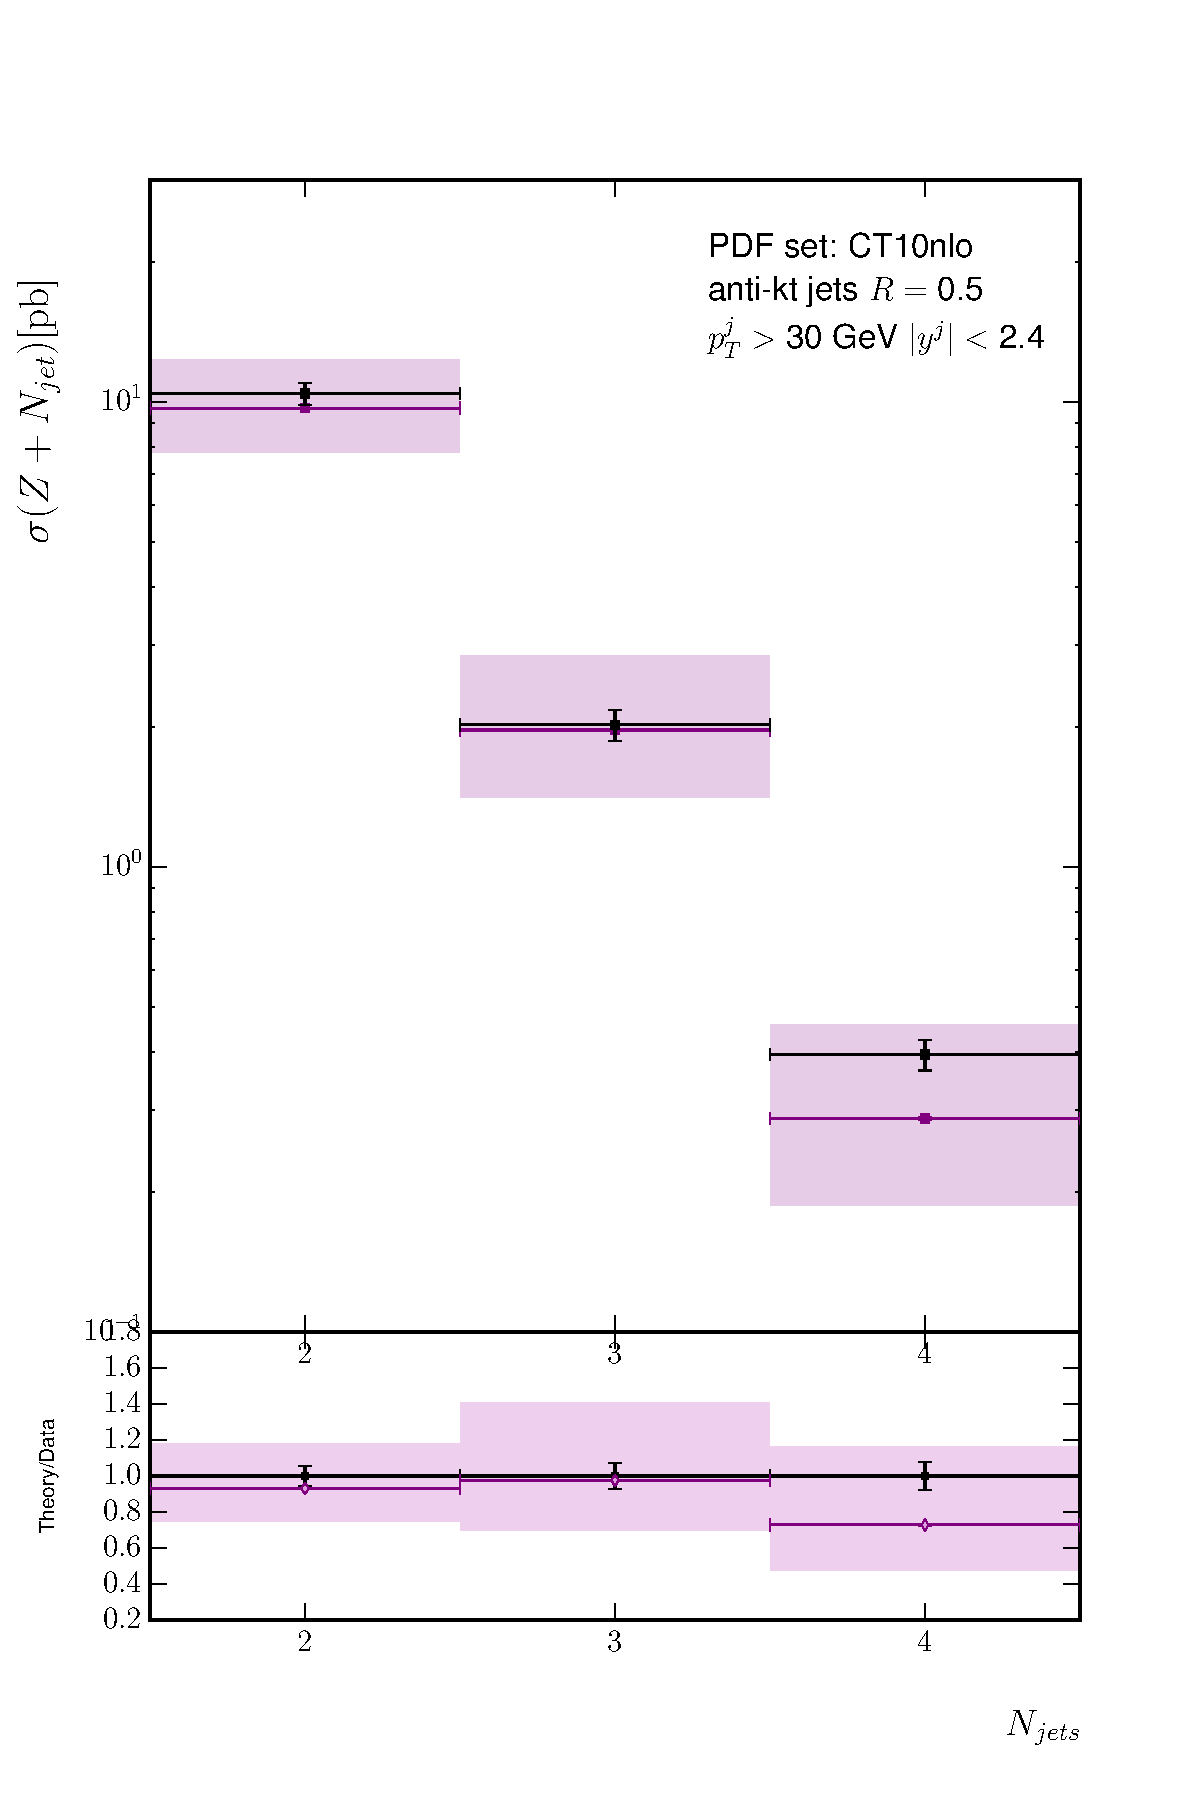
\includegraphics[width=\textwidth, height=1.2\textwidth]{CMS_Z_2a}
		    \caption{}
		    \label{fig:HEJ_CMS_2a}
		  \end{subfigure}
		  ~
		  \begin{subfigure}[b]{0.48\textwidth}
		    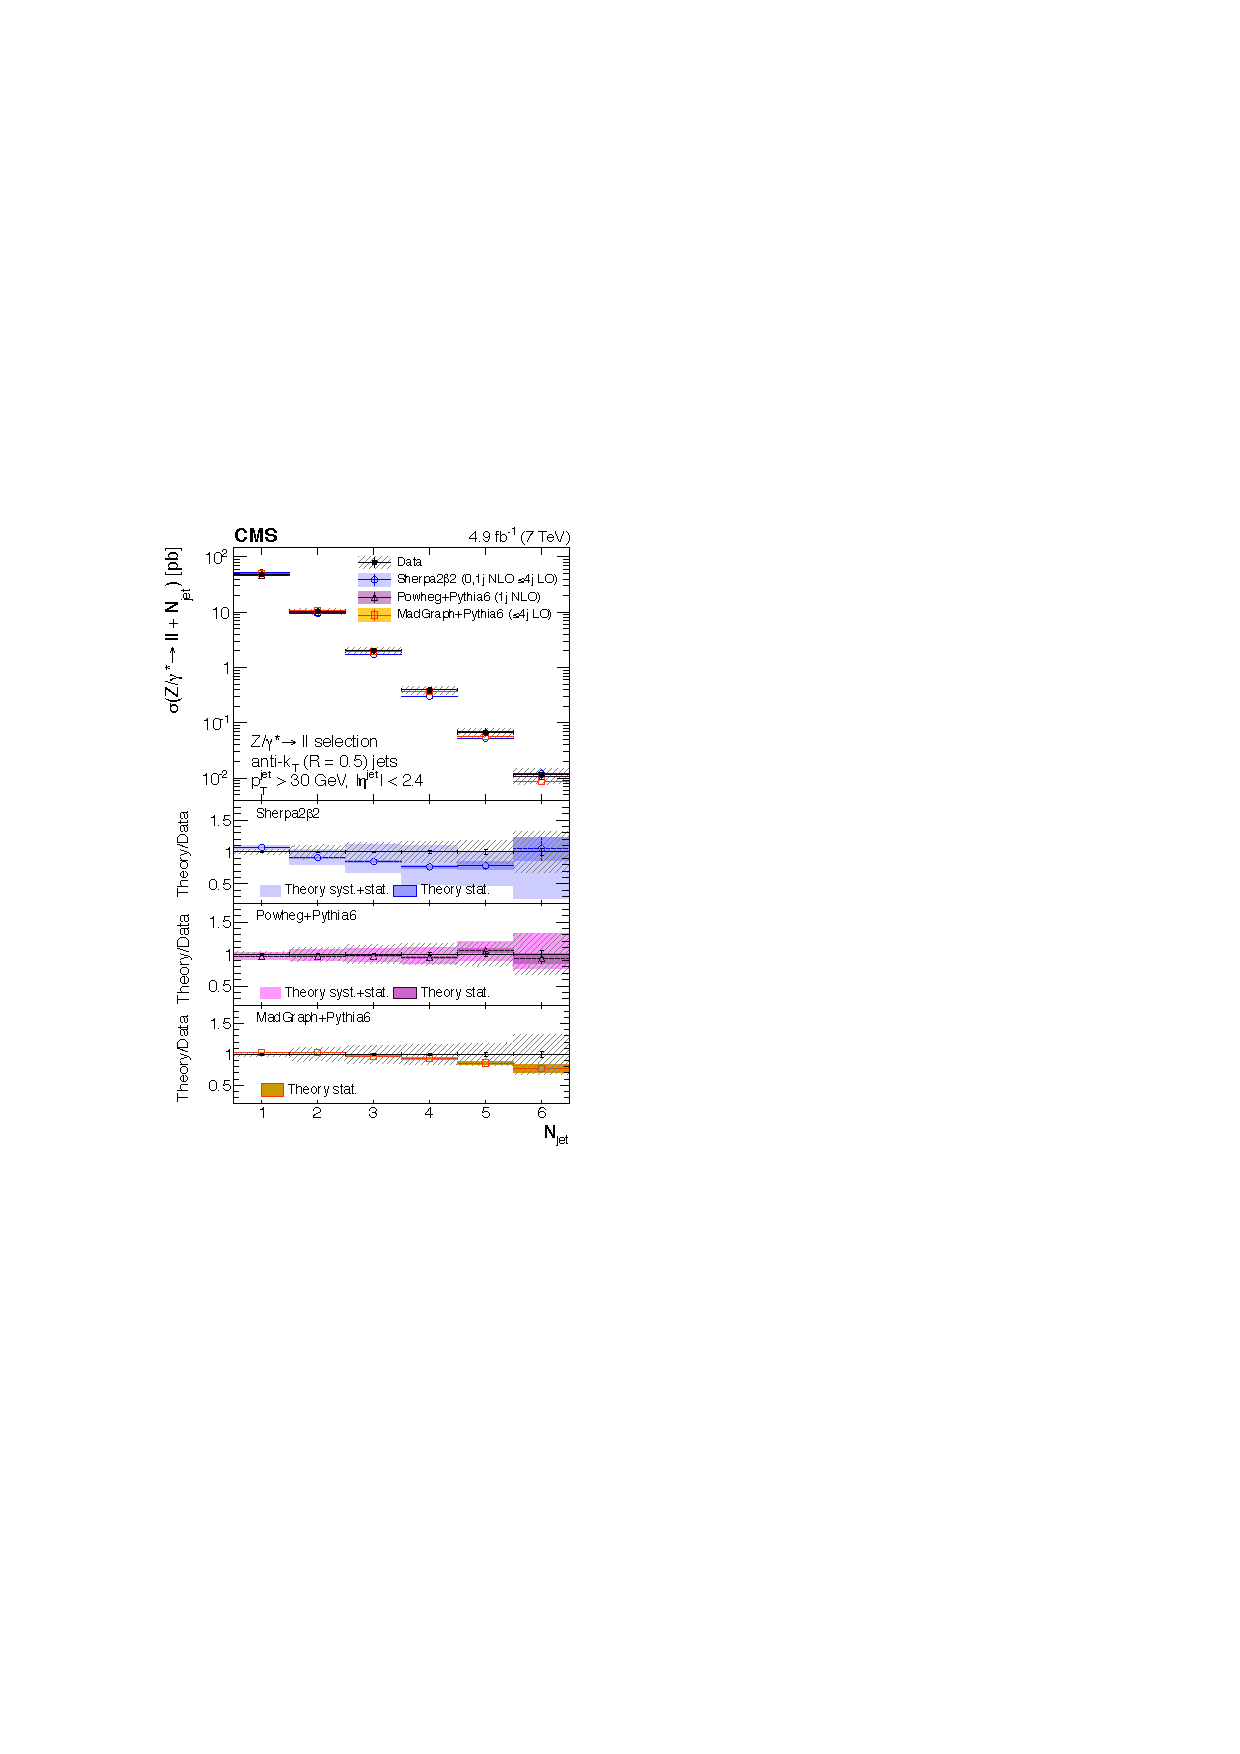
\includegraphics[width=\textwidth, height=1.2\textwidth]{ComparisonCMS_2a}
		    \caption{}
		    \label{fig:MC_CMS_2a}
		  \end{subfigure}
		  \caption{The inclusive jet rates as given by (a) the HEJ description and (b)
		    by other theoretical descriptions, both plots compared to the CMS data in~\cite{Khachatryan:2014zya}.}
		  \label{fig:CMS_2a}

		  \begin{subfigure}[b]{0.46\textwidth}
		    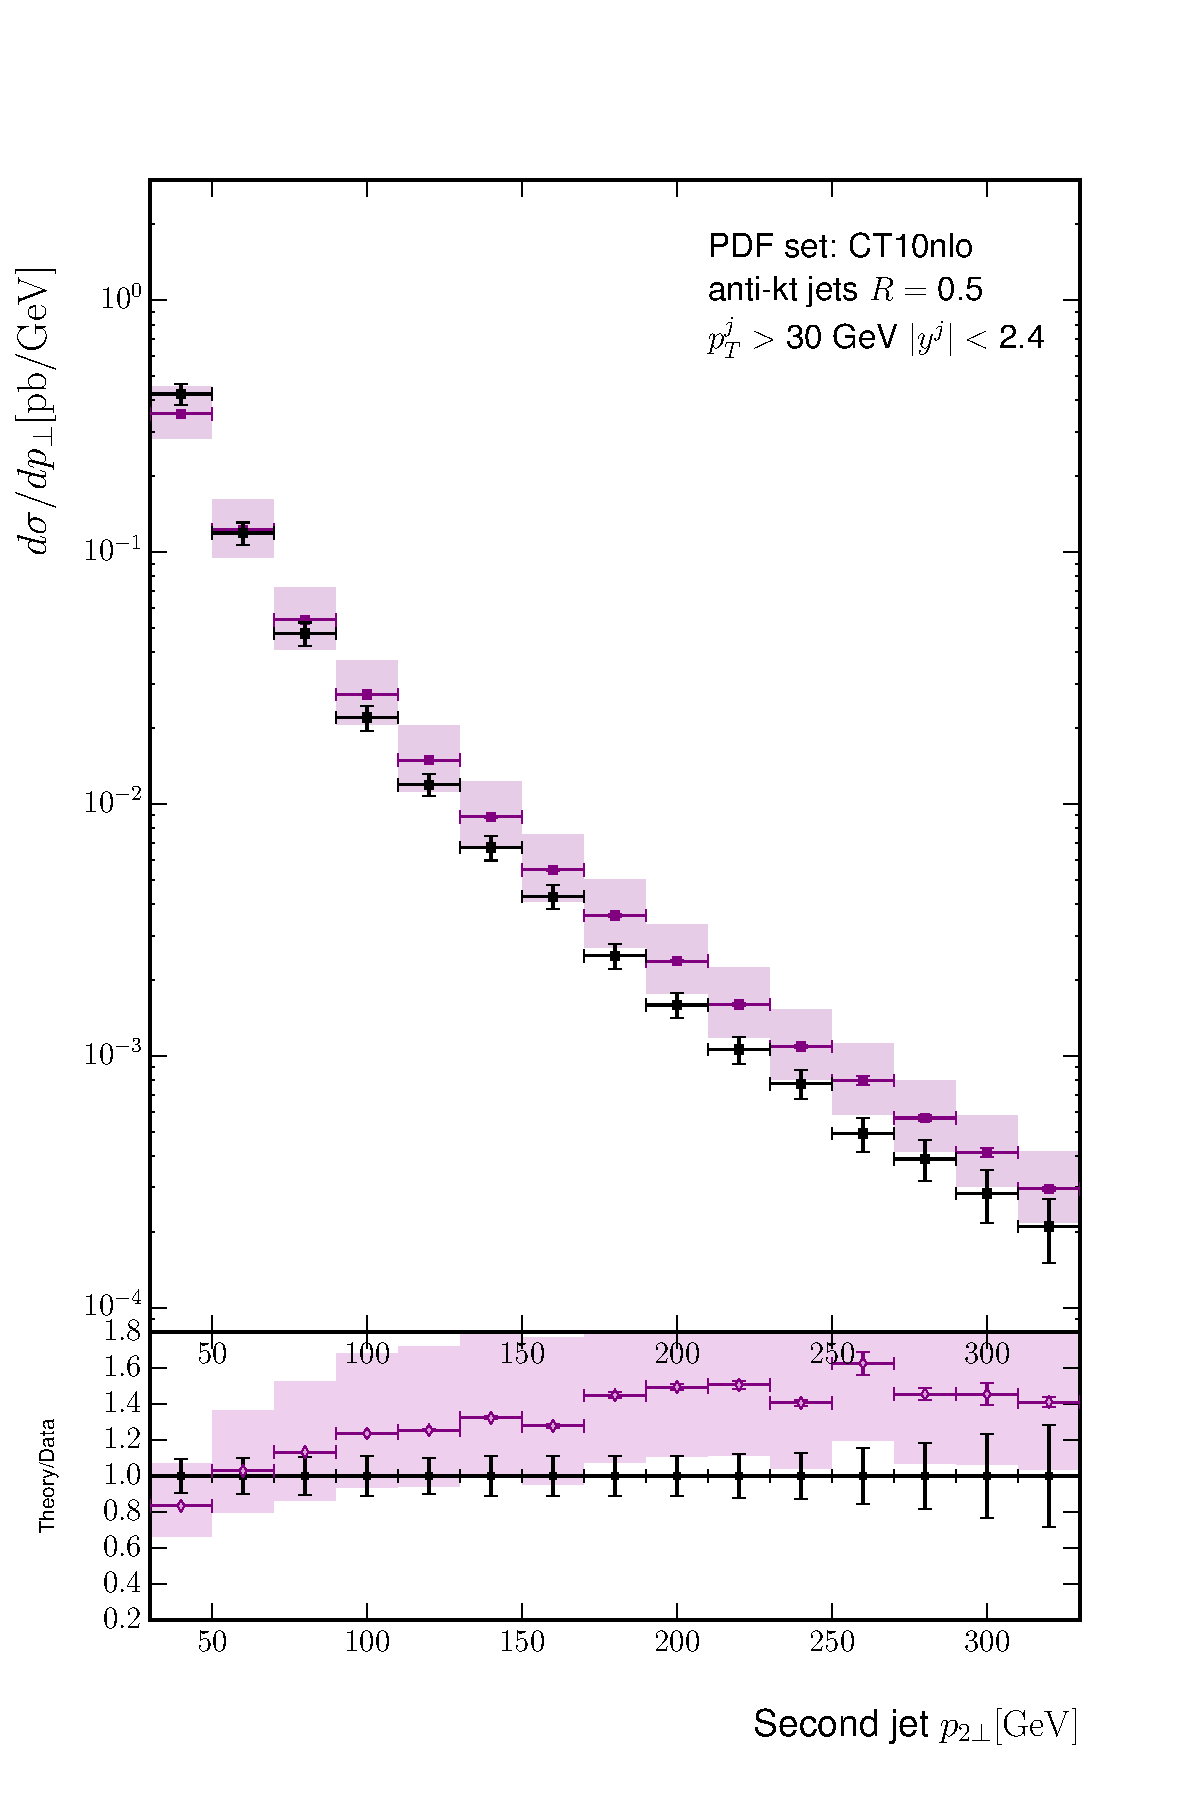
\includegraphics[width=\textwidth, height=1.2\textwidth]{CMS_Z_3b}
		    \caption{}
		    \label{fig:HEJ_CMS_7b}
		  \end{subfigure}
		  ~
		  \begin{subfigure}[b]{0.48\textwidth}
		    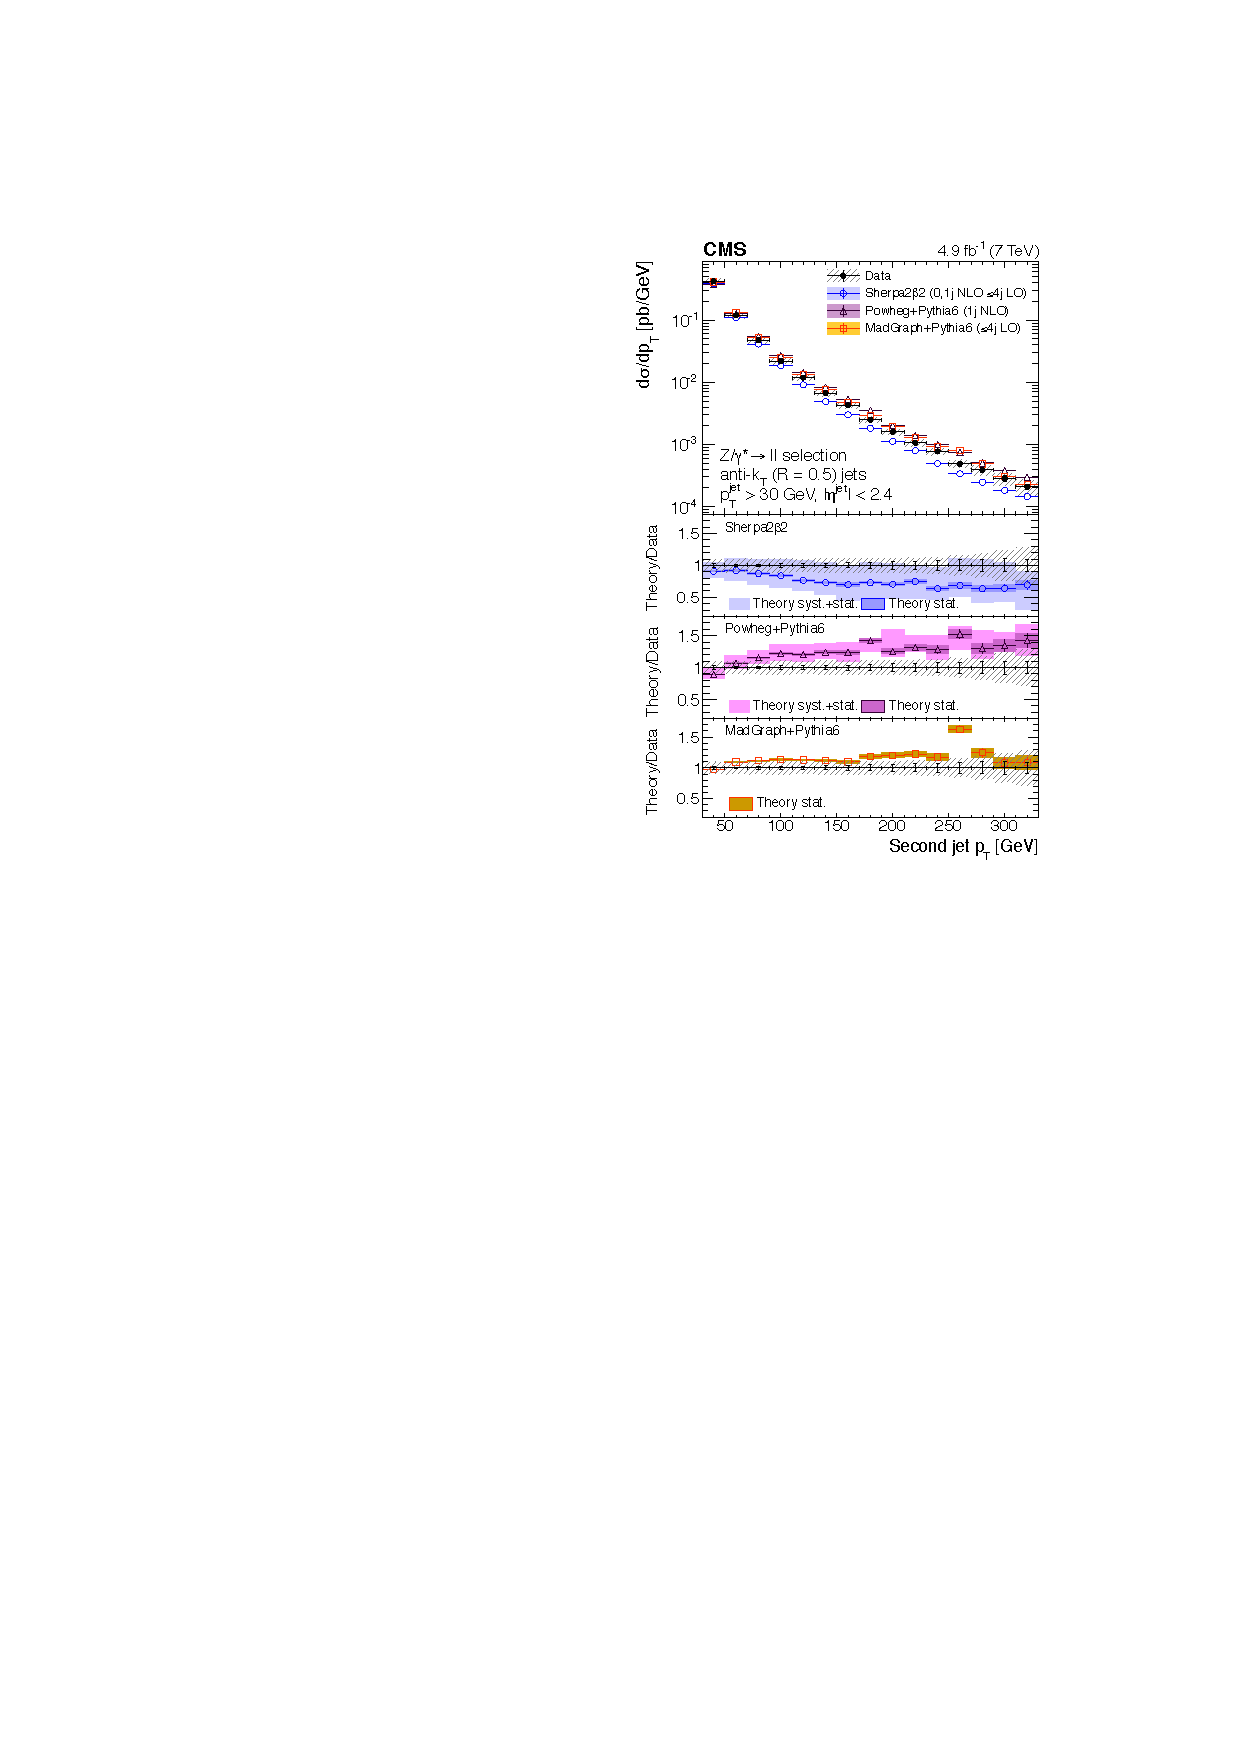
\includegraphics[width=\textwidth, height=1.2\textwidth]{ComparisonCMS_3b}
		    \caption{}
		    \label{fig:MC_CMS_7b}
		  \end{subfigure}
		  \caption{The transverse momentum distribution of the second hardest jet in
		    inclusive dijet events in~\cite{Khachatryan:2014zya}, compared to (a) the
		    predictions from HEJ and (b) the predictions from other theory descriptions.}
		  \label{fig:CMS_3b}
		\end{figure}

		\begin{figure}[H]
		  \centering
		  \begin{subfigure}[b]{0.46\textwidth}
		    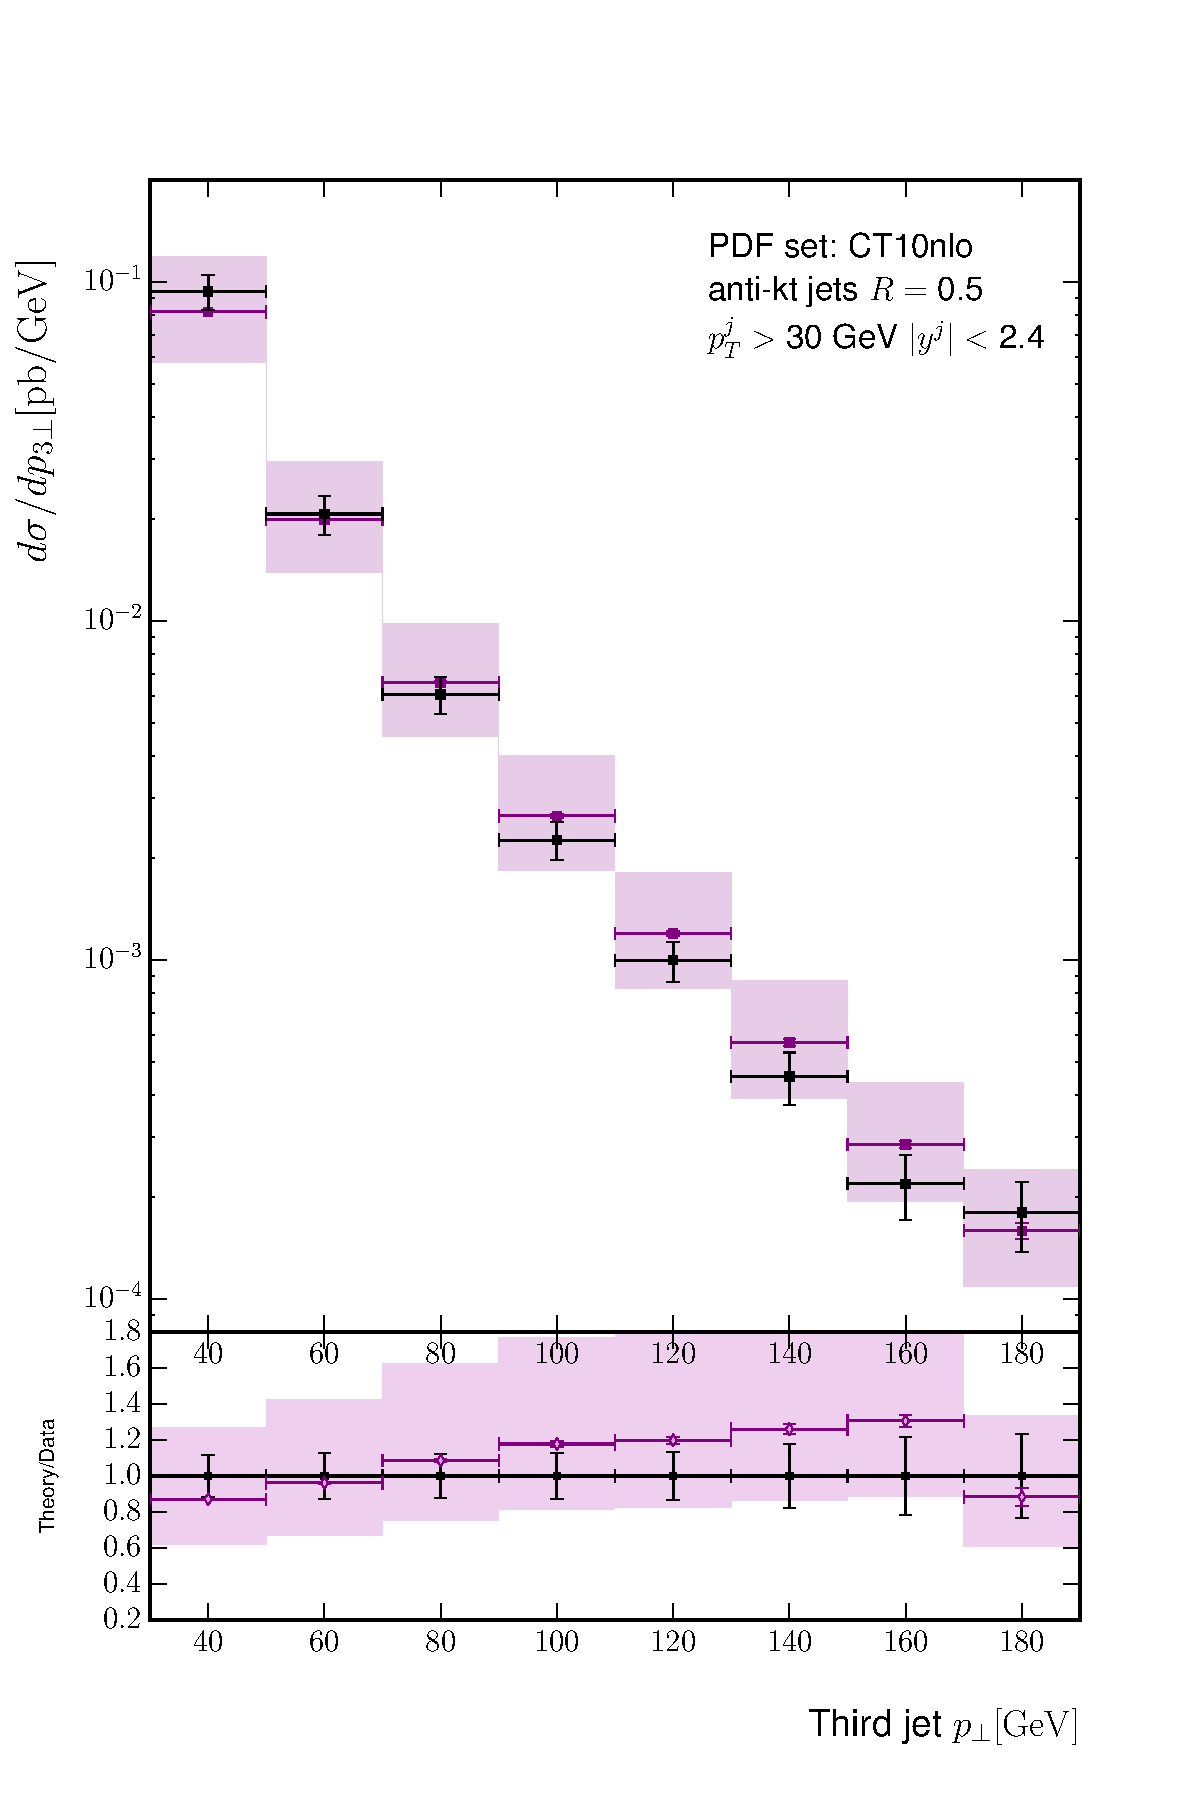
\includegraphics[width=\textwidth, height=1.2\textwidth]{CMS_Z_3c}
		    \caption{}
		    \label{fig:HEJ_CMS_7b}
		  \end{subfigure}
		  ~
		  \begin{subfigure}[b]{0.48\textwidth}
		    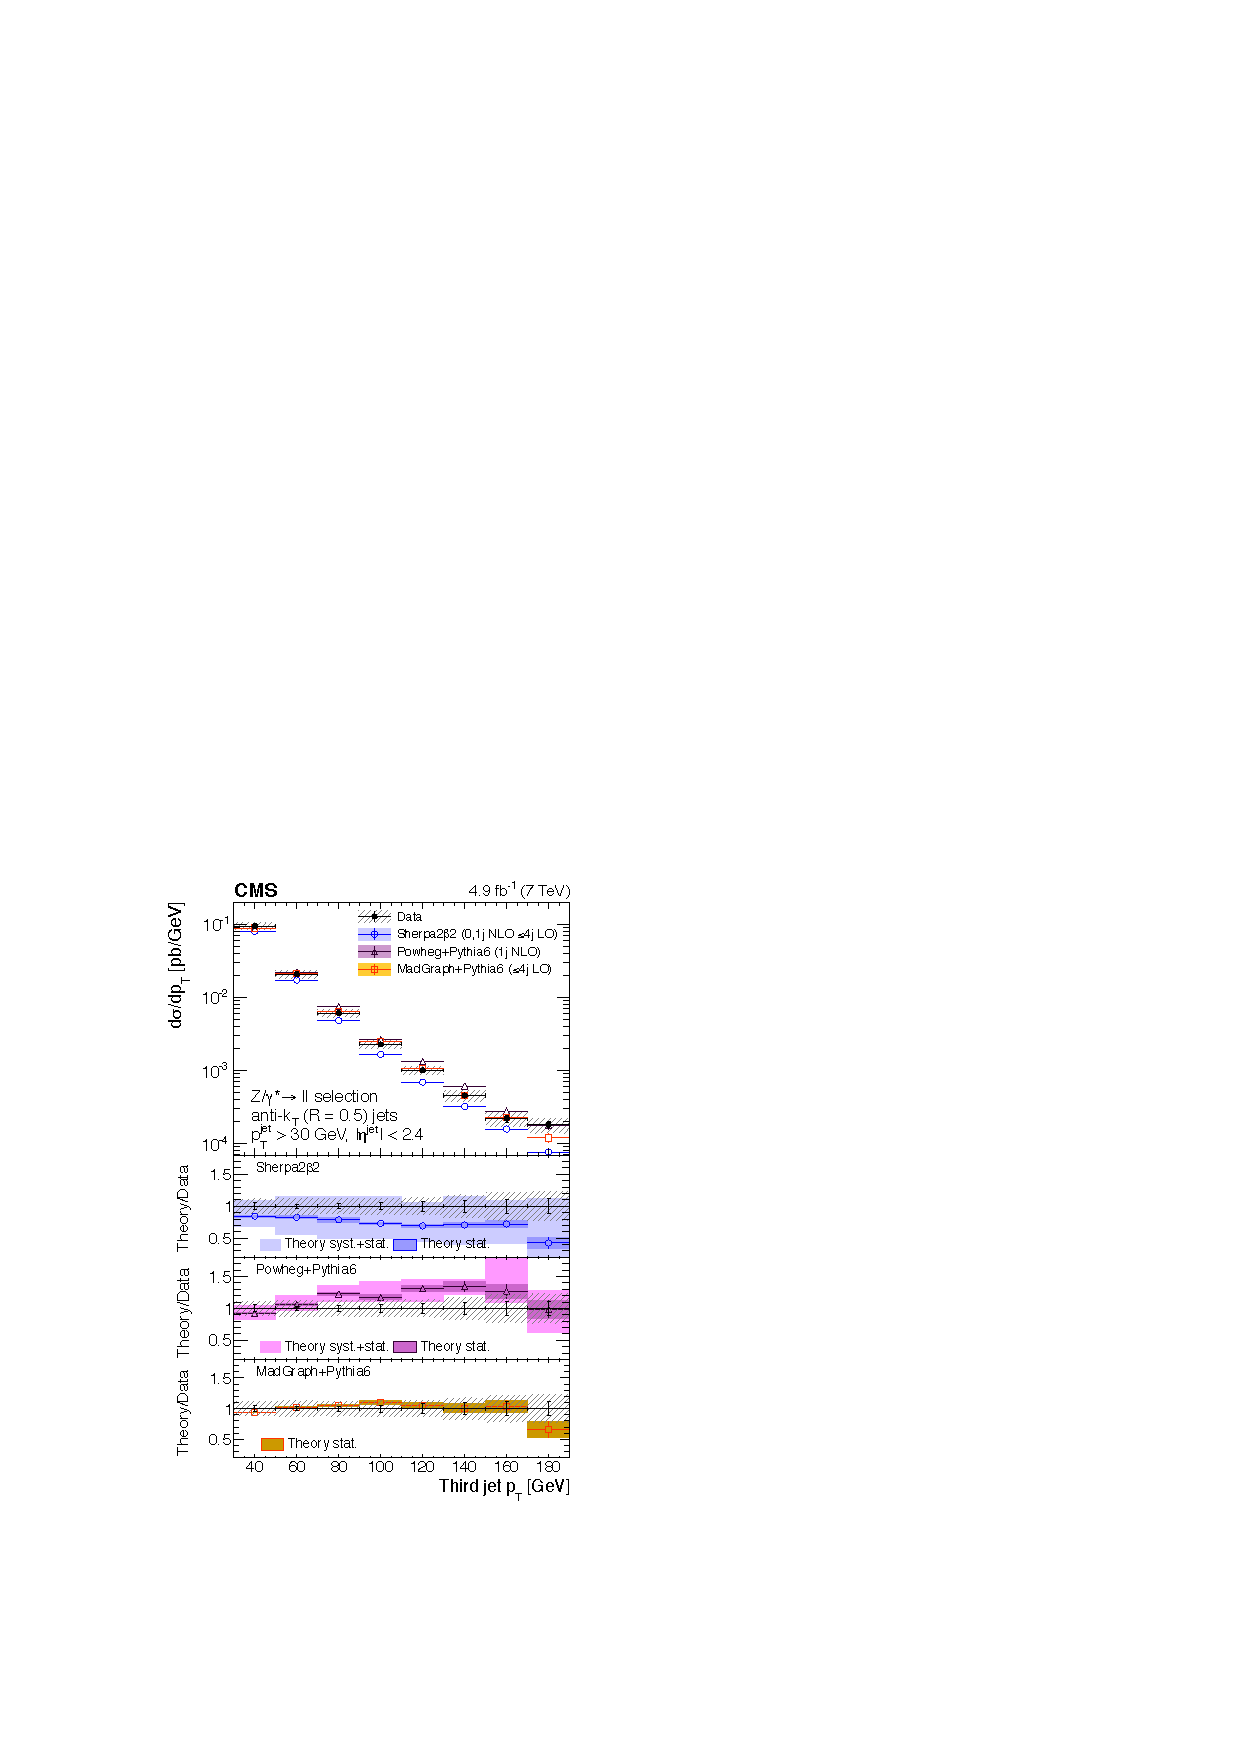
\includegraphics[width=\textwidth, height=1.2\textwidth]{ComparisonCMS_3c}
		    \caption{}
		    \label{fig:MC_CMS_7b}
		  \end{subfigure}
		  \caption{The transverse momentum distribution of the third hardest jet in
		    inclusive dijet events in~\cite{Khachatryan:2014zya}, compared to (a) the
		    predictions from HEJ and (b) the predictions from other theory descriptions.}
		  \label{fig:CMS_3c}
		\end{figure}

